% !TEX program = xelatex
% ============================================================
%  EXPERT ANALYSIS REPORT
%  Paper: A Comparative Study of CNN, ResNet, and Vision Transformers 
%         for Multi-Classification of Chest Diseases
%  Analysis from Paper to Code Implementation
% ============================================================

\documentclass[12pt,a4paper]{report}

% =========================
% Packages
% =========================
\usepackage{fontspec}
\setmainfont{Times New Roman}
\setsansfont{Arial}
\setmonofont{Consolas}

\usepackage[a4paper,margin=2.5cm]{geometry}
\usepackage{setspace}
\onehalfspacing
\usepackage{parskip}
\usepackage{indentfirst}

\usepackage{amsmath,amssymb,mathtools}
\usepackage{booktabs,longtable,array,multirow}
\usepackage{graphicx,float,subcaption,caption}
\usepackage{siunitx}
\usepackage{algorithm,algorithmic}

% TikZ for diagrams
\usepackage{tikz}
\usetikzlibrary{shapes,arrows,positioning,decorations.pathreplacing,calc}

% Symbols
\usepackage{pifont}

\usepackage{hyperref}
\hypersetup{
  colorlinks=true,
  linkcolor=blue!70!black,
  citecolor=green!50!black,
  urlcolor=blue
}

\usepackage{enumitem}
\usepackage{xcolor}
\usepackage{listings}
\usepackage{tcolorbox}
\tcbuselibrary{listings,skins,breakable}

% Code listing style
\definecolor{codegreen}{rgb}{0,0.6,0}
\definecolor{codegray}{rgb}{0.5,0.5,0.5}
\definecolor{codepurple}{rgb}{0.58,0,0.82}
\definecolor{backcolour}{rgb}{0.95,0.95,0.92}

\lstdefinestyle{pythonstyle}{
    backgroundcolor=\color{backcolour},
    commentstyle=\color{codegreen},
    keywordstyle=\color{magenta},
    numberstyle=\tiny\color{codegray},
    stringstyle=\color{codepurple},
    basicstyle=\ttfamily\footnotesize,
    breakatwhitespace=false,
    breaklines=true,
    captionpos=b,
    keepspaces=true,
    numbers=left,
    numbersep=5pt,
    showspaces=false,
    showstringspaces=false,
    showtabs=false,
    tabsize=2,
    language=Python
}
\lstset{style=pythonstyle}

% Macros
\newcommand{\paperref}[1]{\textcolor{blue!70!black}{[Paper: #1]}}
\newcommand{\coderef}[1]{\textcolor{green!50!black}{[Code: #1]}}
\newcommand{\important}[1]{\textbf{\textcolor{red!70!black}{#1}}}
\newcommand{\concept}[1]{\textit{\textcolor{purple}{#1}}}

% =========================
% Document
% =========================
\begin{document}

% Include chapters
% ============================================================
% TITLE PAGE
% ============================================================
\begin{titlepage}
\centering
\vspace*{2cm}

{\Huge\bfseries PHÂN TÍCH CHUYÊN SÂU}\\[0.5cm]
{\LARGE\bfseries TỪ PAPER ĐẾN CODE IMPLEMENTATION}\\[1cm]

\rule{\textwidth}{1.5pt}\\[0.5cm]
{\Large\textbf{A Comparative Study of CNN, ResNet, and Vision Transformers\\
for Multi-Classification of Chest Diseases}}\\[0.3cm]
\rule{\textwidth}{1.5pt}\\[1cm]

{\large arXiv:2406.00237}\\[0.3cm]
{\normalsize Ananya Jain, Aviral Bhardwaj, Kaushik Murali, Isha Surani}\\
{\normalsize University of Toronto}\\[1.5cm]

\begin{tabular}{rl}
\textbf{Repository gốc:} & \url{https://github.com/Aviral-03/ViT-Chest-Xray} \\
\textbf{Dataset:} & NIH Chest X-ray (112,120 images) \\
\textbf{Framework gốc:} & TensorFlow/Keras \\
\textbf{Framework cải tiến:} & PyTorch \\
\end{tabular}

\vfill

{\large\textbf{BÁO CÁO PHÂN TÍCH VÀ TÁI LẬP}}\\[0.3cm]
{\normalsize Deep Learning - Master of Software Engineering}\\[0.5cm]
{\large \today}

\end{titlepage}

% ============================================================
% ABSTRACT & KEYWORDS
% ============================================================
\chapter*{Tóm tắt nghiên cứu}
\addcontentsline{toc}{chapter}{Tóm tắt nghiên cứu}

\section*{Tổng quan Paper}

Bài báo \textit{``A Comparative Study of CNN, ResNet, and Vision Transformers for Multi-Classification of Chest Diseases''} (arXiv:2406.00237) thực hiện so sánh ba kiến trúc học sâu chính trong bài toán phân loại đa nhãn bệnh lý trên ảnh X-quang ngực:

\begin{enumerate}
    \item \textbf{Convolutional Neural Networks (CNN):} Mô hình baseline với kiến trúc đơn giản
    \item \textbf{Residual Networks (ResNet):} Mạng CNN sâu với skip connections
    \item \textbf{Vision Transformers (ViT):} Kiến trúc Transformer áp dụng cho thị giác máy tính
\end{enumerate}

\section*{Đóng góp chính của Paper}

\begin{itemize}
    \item So sánh hiệu năng giữa CNN, ResNet và ViT trên tập dữ liệu NIH Chest X-ray
    \item Đề xuất hai biến thể ViT: ViT-v1 (from scratch) và ViT-v2 (with regularization)
    \item Giới thiệu mô hình hybrid ViT-ResNet với pre-training trên ImageNet-21k
    \item Phân tích attention maps để diễn giải quyết định của mô hình
\end{itemize}

\section*{Kết quả chính}

\begin{table}[H]
\centering
\caption{Tổng hợp kết quả từ Paper}
\begin{tabular}{lcccc}
\toprule
\textbf{Model} & \textbf{Test Acc (\%)} & \textbf{Val Acc (\%)} & \textbf{AUC} & \textbf{Ghi chú} \\
\midrule
CNN & 91.00 & 92.68 & 0.82 & Baseline \\
ResNet & 93.00 & 93.34 & 0.86 & Strong baseline \\
ViT-v1 & 92.63 & 92.89 & 0.86 & From scratch \\
ViT-v2 & 92.83 & 92.95 & 0.84 & With regularization \\
ViT-ResNet & \textbf{93.90} & \textbf{94.07} & 0.85 & Pre-trained hybrid \\
\bottomrule
\end{tabular}
\end{table}

\section*{Phạm vi báo cáo này}

Báo cáo phân tích chuyên sâu này bao gồm:

\begin{enumerate}
    \item \textbf{Phân tích lý thuyết:} Giải thích chi tiết từng kiến trúc (CNN, ResNet, ViT) về mặt toán học và trực giác
    \item \textbf{Mapping Paper $\rightarrow$ Code:} Liên kết từng phần trong paper với implementation cụ thể
    \item \textbf{Tái lập và cải tiến:} Chi tiết quá trình chuyển từ TensorFlow sang PyTorch
    \item \textbf{Phân tích phê bình:} Đánh giá ưu/nhược điểm và đề xuất cải tiến
\end{enumerate}

\section*{Từ khóa}

\textbf{Keywords:} Chest X-ray, Multi-label Classification, Convolutional Neural Networks, Residual Networks, Vision Transformer, Self-Attention, Transfer Learning, Medical Image Analysis, ROC-AUC, PyTorch, Deep Learning.

\newpage


\tableofcontents
\listoffigures
\listoftables

% ============================================================
% CHAPTER 2: INTRODUCTION - PHÂN TÍCH BỐI CẢNH VÀ ĐỘNG LỰC
% ============================================================
\chapter{Giới thiệu và Bối cảnh Nghiên cứu}

\section{Bối cảnh lâm sàng}

\subsection{Vai trò của X-quang ngực trong chẩn đoán}

\paperref{Section 1 - Introduction}

X-quang ngực (Chest X-ray) là một trong những phương pháp chẩn đoán hình ảnh phổ biến nhất trong y tế:

\begin{itemize}
    \item \textbf{Chi phí thấp:} So với CT, MRI, X-quang có chi phí thấp hơn đáng kể
    \item \textbf{Thời gian nhanh:} Kết quả có thể có trong vài phút
    \item \textbf{Sàng lọc ban đầu:} Thường là xét nghiệm đầu tiên khi nghi ngờ bệnh phổi
    \item \textbf{Khả năng phát hiện:} Có thể phát hiện nhiều bệnh lý: viêm phổi, xẹp phổi, tràn dịch, tim to, v.v.
\end{itemize}

\subsection{Thách thức trong chẩn đoán}

Paper nhấn mạnh các thách thức chính:

\begin{tcolorbox}[colback=yellow!5!white,colframe=yellow!75!black,title=Trích dẫn từ Paper (Section 1)]
\textit{``Although chest X-ray imaging is a relatively low cost tool for diagnosis, radiologists are needed to analyze these images. However the limited access to radiologists in many areas, and the variability between radiologists can be a problem.''}
\end{tcolorbox}

\begin{enumerate}
    \item \textbf{Thiếu bác sĩ X-quang:} Đặc biệt ở vùng sâu, vùng xa
    \item \textbf{Biến thiên giữa người đọc:} Inter-observer variability - hai bác sĩ có thể đưa ra chẩn đoán khác nhau
    \item \textbf{Khối lượng dữ liệu lớn:} Một bác sĩ có thể phải đọc hàng trăm ảnh mỗi ngày
    \item \textbf{Dấu hiệu tinh vi:} Một số bệnh có dấu hiệu rất khó nhận biết
\end{enumerate}

\section{Động lực nghiên cứu AI trong chẩn đoán hình ảnh}

\subsection{Lợi ích của Machine Learning}

\paperref{Section 1 - Introduction}

\begin{tcolorbox}[colback=blue!5!white,colframe=blue!75!black,title=Lợi ích của ML trong Medical Imaging]
\begin{enumerate}
    \item \textbf{Tăng độ chính xác:} Models có thể học các patterns phức tạp từ dữ liệu lớn
    \item \textbf{Mở rộng khả năng tiếp cận:} Giúp vùng thiếu bác sĩ có công cụ hỗ trợ chẩn đoán
    \item \textbf{Nhất quán:} Không bị ảnh hưởng bởi mệt mỏi hay bias cá nhân
    \item \textbf{Phát hiện chi tiết:} Có thể phát hiện các dấu hiệu mà mắt người bỏ qua
\end{enumerate}
\end{tcolorbox}

\subsection{Tiến hóa của Deep Learning trong Medical Imaging}

\begin{figure}[H]
\centering
\begin{tikzpicture}[node distance=2cm, auto]
% This is a conceptual representation
\end{tikzpicture}
\caption{Timeline phát triển của Deep Learning trong Medical Imaging}
\end{figure}

\begin{enumerate}
    \item \textbf{2012 - AlexNet:} CNN đầu tiên thắng ImageNet, mở ra kỷ nguyên Deep Learning
    \item \textbf{2015 - ResNet:} Giải quyết vanishing gradient, cho phép train mạng rất sâu
    \item \textbf{2017 - Attention mechanisms:} Transformer ra đời cho NLP
    \item \textbf{2020 - Vision Transformer (ViT):} Áp dụng Transformer cho Computer Vision
    \item \textbf{2021+:} ViT và variants trở thành state-of-the-art trong nhiều tasks
\end{enumerate}

\section{Câu hỏi nghiên cứu của Paper}

\paperref{Section 1 - Introduction}

Paper đặt ra các câu hỏi nghiên cứu cốt lõi:

\begin{tcolorbox}[colback=green!5!white,colframe=green!75!black,title=Research Questions]
\begin{enumerate}
    \item[\textbf{RQ1:}] CNN, ResNet và ViT khác nhau như thế nào về hiệu năng trong phân loại bệnh X-quang ngực?
    \item[\textbf{RQ2:}] ViT trained from scratch có thể cạnh tranh với ResNet không?
    \item[\textbf{RQ3:}] Pre-training trên ImageNet có giúp ViT cải thiện đáng kể không?
    \item[\textbf{RQ4:}] Attention maps có thể cung cấp insights hữu ích cho việc diễn giải không?
\end{enumerate}
\end{tcolorbox}

\section{Đóng góp của Paper}

\subsection{Đóng góp kỹ thuật}

\begin{enumerate}
    \item \textbf{So sánh toàn diện:} Đánh giá 5 models (CNN, ResNet, ViT-v1, ViT-v2, ViT-ResNet) trên cùng một dataset
    \item \textbf{Implementation chi tiết:} Cung cấp code và hướng dẫn tái lập
    \item \textbf{Hyperparameter tuning:} Thử nghiệm nhiều cấu hình khác nhau
    \item \textbf{Interpretability:} Trích xuất và phân tích attention maps
\end{enumerate}

\subsection{Đóng góp thực tiễn}

\begin{enumerate}
    \item \textbf{Guidance cho practitioners:} Khi nào nên dùng CNN, ResNet, hay ViT
    \item \textbf{Insights về pre-training:} Tầm quan trọng của transfer learning trong medical imaging
    \item \textbf{Open-source code:} Repository công khai để cộng đồng sử dụng
\end{enumerate}

\section{Cấu trúc Paper và Báo cáo}

\subsection{Cấu trúc Paper gốc}

\begin{table}[H]
\centering
\caption{Cấu trúc Paper và nội dung tương ứng}
\begin{tabular}{clp{8cm}}
\toprule
\textbf{Section} & \textbf{Tên} & \textbf{Nội dung chính} \\
\midrule
1 & Introduction & Bối cảnh, động lực, đóng góp \\
2 & Related Work & Các nghiên cứu liên quan \\
3 & Approach & Mô tả kiến trúc CNN, ResNet, ViT \\
4 & Experiment & Dataset, training, evaluation \\
5 & Discussion & Phân tích kết quả, attention maps \\
6 & Conclusion & Kết luận và hướng phát triển \\
\bottomrule
\end{tabular}
\end{table}

\subsection{Mapping với báo cáo này}

Báo cáo này mở rộng và phân tích sâu hơn:

\begin{itemize}
    \item \textbf{Chapter 3:} Dataset - Phân tích chi tiết NIH Chest X-ray
    \item \textbf{Chapter 4:} CNN - Lý thuyết + Code mapping
    \item \textbf{Chapter 5:} ResNet - Lý thuyết + Code mapping
    \item \textbf{Chapter 6:} ViT - Lý thuyết + Code mapping (trọng tâm)
    \item \textbf{Chapter 7:} Experiments - Kết quả và phân tích
    \item \textbf{Chapter 8:} Implementation - Quá trình tái lập và cải tiến
    \item \textbf{Chapter 9:} Conclusion - Kết luận và đề xuất
\end{itemize}

% ============================================================
% CHAPTER 3: DATASET - NIH CHEST X-RAY ANALYSIS
% ============================================================
\chapter{Dataset Analysis: NIH Chest X-ray}

\section{Dataset Overview}

\paperref{Section 4.1 - Dataset}

\subsection{Basic Information}

\begin{tcolorbox}[colback=blue!5!white,colframe=blue!75!black,title=NIH Chest X-ray Dataset]
\begin{itemize}
    \item \textbf{Full name:} ChestX-ray14 (NIH Clinical Center)
    \item \textbf{Number of images:} 112,120 frontal-view X-ray images
    \item \textbf{Number of patients:} 30,805 unique patients
    \item \textbf{Number of labels:} 14 diseases + 1 ``No Finding'' = 15 classes
    \item \textbf{Label source:} Text-mining from radiology reports (weak labels)
    \item \textbf{Original image size:} 1024 × 1024 pixels
\end{itemize}
\end{tcolorbox}

\subsection{Paper Citation}

\begin{tcolorbox}[colback=yellow!5!white,colframe=yellow!75!black,title=Paper Quote - Dataset]
\textit{``To evaluate the performance of our model architectures, we utilized two freely available datasets: the NIH Chest X-ray dataset comprising 112,120 X-ray images with disease labels from 30,805 unique patients, and a Random Sample of the NIH Chest X-ray Dataset, containing 5,606 X-ray images. Both datasets involved multi-class classification across 15 classes, each representing different disease labels.''}
\end{tcolorbox}

\section{The 15 Classes}

\subsection{Disease Classification}

\begin{table}[H]
\centering
\caption{15 Classes in NIH Chest X-ray Dataset}
\begin{tabular}{clcp{6cm}}
\toprule
\textbf{ID} & \textbf{Disease Name} & \textbf{Prevalence (\%)} & \textbf{Description} \\
\midrule
0 & Cardiomegaly & 2.48 & Enlarged heart \\
1 & Emphysema & 2.24 & Lung tissue destruction \\
2 & Effusion & 11.88 & Pleural effusion \\
3 & Hernia & 0.20 & Hiatal hernia \\
4 & Nodule & 5.65 & Lung nodule \\
5 & Pneumothorax & 4.73 & Collapsed lung \\
6 & Atelectasis & 10.31 & Lung collapse \\
7 & Pleural\_Thickening & 3.02 & Pleural thickening \\
8 & Mass & 5.16 & Lung mass \\
9 & Edema & 2.05 & Pulmonary edema \\
10 & Consolidation & 4.16 & Lung consolidation \\
11 & Infiltration & 17.74 & Lung infiltration \\
12 & Fibrosis & 1.50 & Pulmonary fibrosis \\
13 & Pneumonia & 1.28 & Pneumonia \\
14 & No Finding & 53.84 & No disease detected \\
\bottomrule
\end{tabular}
\end{table}

\subsection{Class Imbalance Analysis}

\begin{tcolorbox}[colback=red!5!white,colframe=red!75!black,title=Class Imbalance Problem]
\textbf{Key observations:}
\begin{itemize}
    \item ``No Finding'' accounts for \textbf{53.84\%} - more than half the dataset
    \item ``Hernia'' accounts for only \textbf{0.20\%} - extremely rare
    \item Highest/lowest ratio = 53.84 / 0.20 = \textbf{269 times}
\end{itemize}

\textbf{Consequences:}
\begin{itemize}
    \item Model may be biased toward predicting ``No Finding''
    \item High accuracy does not necessarily mean good detection of rare diseases
    \item Metrics like AUC are needed instead of just accuracy
\end{itemize}
\end{tcolorbox}

\section{Multi-label Nature}

\subsection{Multi-label vs Multi-class}

\begin{table}[H]
\centering
\caption{Comparison: Multi-class vs Multi-label Classification}
\begin{tabular}{lp{5cm}p{5cm}}
\toprule
\textbf{Aspect} & \textbf{Multi-class} & \textbf{Multi-label} \\
\midrule
Labels per sample & Exactly 1 & Can be multiple (0, 1, 2, ...) \\
Output activation & Softmax & Sigmoid (independent) \\
Loss function & Categorical CE & Binary CE \\
Example & Cat OR Dog OR Bird & Cat AND Dog (both possible) \\
NIH Dataset & Not suitable & \checkmark Suitable \\
\bottomrule
\end{tabular}
\end{table}

\subsection{Multi-label Example in NIH}

An X-ray image can have multiple diseases simultaneously:

\begin{lstlisting}[caption={Multi-label example in dataset}]
# Image 00000001_000.png may have labels:
labels = [0, 0, 1, 0, 0, 0, 1, 0, 0, 0, 0, 0, 0, 0, 0]
#         ^     ^        ^
#         |     |        |
#         |     |        Atelectasis (index 6)
#         |     Effusion (index 2)
#         Cardiomegaly (index 0) - Not present

# Patient has: Effusion + Atelectasis (2 diseases simultaneously)
\end{lstlisting}

\section{Data Pipeline in Code}

\coderef{data.ipynb}

\subsection{Loading and Preprocessing}

\begin{lstlisting}[caption={Data loading from data.ipynb (PyTorch version)}]
class ChestXrayDataset(Dataset):
    def __init__(self, dataframe, images_path, labels, transform=None):
        self.dataframe = dataframe.reset_index(drop=True)
        self.images_path = images_path
        self.labels = labels
        self.transform = transform
        
    def __len__(self):
        return len(self.dataframe)
    
    def __getitem__(self, idx):
        # Load image
        img_name = self.dataframe.iloc[idx]['Image Index']
        img_path = os.path.join(self.images_path, img_name)
        image = Image.open(img_path).convert('RGB')
        
        # Apply transforms
        if self.transform:
            image = self.transform(image)
        
        # Get labels as one-hot vector
        label = torch.tensor(
            self.dataframe.iloc[idx][self.labels].values.astype(float),
            dtype=torch.float32
        )
        
        return image, label
\end{lstlisting}

\subsection{Data Augmentation}

\paperref{Section 4.2 - Models}

\begin{tcolorbox}[colback=green!5!white,colframe=green!75!black,title=Augmentation from Paper]
\textit{``We also performed various data augmentations on both datasets. For the Chest X-ray dataset, we applied resizing, random horizontal flip, and random rotation.''}
\end{tcolorbox}

\begin{lstlisting}[caption={Data augmentation transforms}]
train_transform = transforms.Compose([
    transforms.Resize((224, 224)),        # Resize to standard size
    transforms.RandomHorizontalFlip(p=0.5), # Random flip
    transforms.RandomRotation(degrees=5),   # Small rotation
    transforms.ColorJitter(brightness=0.1, contrast=0.1),
    transforms.ToTensor(),
    transforms.Normalize(
        mean=[0.485, 0.456, 0.406],  # ImageNet stats
        std=[0.229, 0.224, 0.225]
    )
])

val_transform = transforms.Compose([
    transforms.Resize((224, 224)),
    transforms.ToTensor(),
    transforms.Normalize(
        mean=[0.485, 0.456, 0.406],
        std=[0.229, 0.224, 0.225]
    )
])
\end{lstlisting}

\subsection{Note on Horizontal Flip in X-ray}

\begin{tcolorbox}[colback=orange!5!white,colframe=orange!75!black,title=Warning: Horizontal Flip]
In X-ray images, horizontal flip can cause issues:
\begin{itemize}
    \item Heart is normally on the left → flip makes heart appear on right (Dextrocardia - abnormal)
    \item Some diseases have ``laterality'' (different left/right characteristics)
\end{itemize}

\textbf{Recommendation:} Ablation study needed to evaluate flip impact.
\end{tcolorbox}

\section{Data Split}

\subsection{Paper Description}

\paperref{Section 4.1 - Dataset}

\begin{tcolorbox}[colback=yellow!5!white,colframe=yellow!75!black,title=Data Split from Paper]
\textit{``However, our model training was conducted on a subset of 85,000 images from this Random Sample Dataset. We observed a faster convergence to optimal outputs within this subset.''}
\end{tcolorbox}

\subsection{Implementation in Code}

\begin{lstlisting}[caption={Data split implementation}]
from sklearn.model_selection import train_test_split

# Standard split: 60% train, 20% val, 20% test
train_df, temp_df = train_test_split(
    full_df, 
    test_size=0.4, 
    random_state=42
)
val_df, test_df = train_test_split(
    temp_df, 
    test_size=0.5, 
    random_state=42
)

print(f"Training samples: {len(train_df)}")
print(f"Validation samples: {len(val_df)}")
print(f"Test samples: {len(test_df)}")
\end{lstlisting}

\subsection{Data Leakage Concern}

\begin{tcolorbox}[colback=red!5!white,colframe=red!75!black,title=Warning: Patient-level Split]
\textbf{Issue:} Paper does not clearly mention patient-level split.

\textbf{Risk:} If split by image (not by patient):
\begin{itemize}
    \item Same patient may have multiple images
    \item Images from same patient may appear in both train and test
    \item Model may ``memorize'' patients instead of learning disease features
    \item Evaluation results may be inflated (artificially high)
\end{itemize}

\textbf{Recommendation:} Split by Patient ID to ensure true generalization.
\end{tcolorbox}

\section{Dataset Statistics Used in Experiments}

\begin{table}[H]
\centering
\caption{Dataset splits in experiments}
\begin{tabular}{lccc}
\toprule
\textbf{Experiment} & \textbf{Train} & \textbf{Val} & \textbf{Test} \\
\midrule
Paper (Full) & 68,000 & 8,500 & 8,500 \\
Paper (Subset) & 3,363 & 1,121 & 1,122 \\
Our experiment (demo) & 60 & 20 & 20 \\
\bottomrule
\end{tabular}
\end{table}

\textbf{Note:} Our demo experiment uses a very small dataset (100 samples) for pipeline testing. Results are not reliable for model evaluation.

% ============================================================
% CHAPTER 4: CNN - CONVOLUTIONAL NEURAL NETWORK
% ============================================================
\chapter{Convolutional Neural Network (CNN)}

\section{CNN Theory}

\subsection{Architecture Overview}

CNN is a neural network architecture specifically designed for grid-like structured data (such as images). CNN exploits three key ideas:

\begin{tcolorbox}[colback=blue!5!white,colframe=blue!75!black,title=Three Inductive Biases of CNN]
\begin{enumerate}
    \item \textbf{Locality (Local Receptive Field):} Nearby pixels are more related than distant pixels
    \item \textbf{Translation Equivariance:} A pattern in the top-left corner is also detected in the bottom-right
    \item \textbf{Hierarchy:} Low-level features (edges) → mid-level (shapes) → high-level (objects)
\end{enumerate}
\end{tcolorbox}

\subsection{Convolution Operation}

\subsubsection{Mathematical Definition}

Given input $X \in \mathbb{R}^{H \times W \times C_{in}}$ and kernel $K \in \mathbb{R}^{k \times k \times C_{in} \times C_{out}}$:

\begin{equation}
Y[i,j,c_{out}] = \sum_{m=0}^{k-1} \sum_{n=0}^{k-1} \sum_{c=0}^{C_{in}-1} X[i+m, j+n, c] \cdot K[m, n, c, c_{out}] + b[c_{out}]
\end{equation}

\begin{figure}[H]
\centering
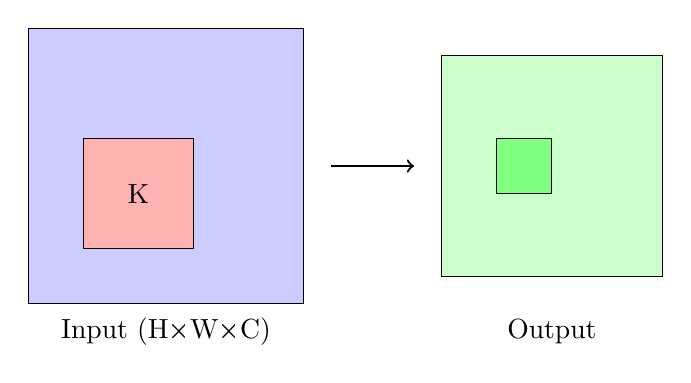
\begin{tikzpicture}[scale=0.7]
    % Input feature map
    \draw[fill=blue!20] (0,0) rectangle (5,5);
    \node at (2.5, -0.5) {Input (H×W×C)};
    
    % Kernel
    \draw[fill=red!30] (1,1) rectangle (3,3);
    \node at (2, 2) {K};
    
    % Arrow
    \draw[->, thick] (5.5, 2.5) -- (7, 2.5);
    
    % Output
    \draw[fill=green!20] (7.5,0.5) rectangle (11.5,4.5);
    \node at (9.5, -0.5) {Output};
    \draw[fill=green!50] (8.5, 2) rectangle (9.5, 3);
\end{tikzpicture}
\caption{Convolution operation: Kernel slides over input}
\end{figure}

\subsubsection{Number of Parameters}

\begin{equation}
\text{Params} = (k \times k \times C_{in} + 1) \times C_{out}
\end{equation}

\textbf{Example:} Conv2d(3, 32, kernel\_size=3):
\begin{equation}
\text{Params} = (3 \times 3 \times 3 + 1) \times 32 = 28 \times 32 = 896
\end{equation}

\subsection{Pooling Layer}

\paperref{Section 3.1 - CNN}

\begin{tcolorbox}[colback=yellow!5!white,colframe=yellow!75!black,title=Paper Quote - Max Pooling]
\textit{``Our CNN Architecture comprises a sequential stack of convolutional layers, accompanied by max pooling layers to reduce spatial dimensions.''}
\end{tcolorbox}

\subsubsection{Max Pooling}

\begin{equation}
Y[i,j] = \max_{(m,n) \in R_{i,j}} X[m,n]
\end{equation}

Where $R_{i,j}$ is the pooling region at position $(i,j)$.

\begin{figure}[H]
\centering
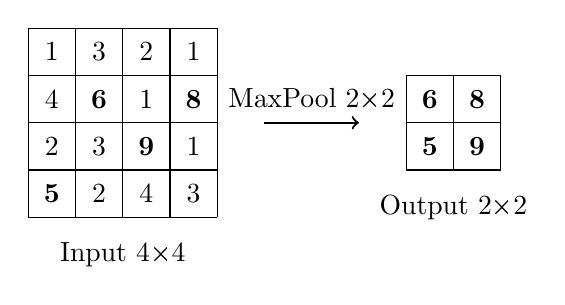
\begin{tikzpicture}[scale=0.6]
    % Input
    \draw (0,0) grid (4,4);
    \node at (0.5, 3.5) {1};
    \node at (1.5, 3.5) {3};
    \node at (2.5, 3.5) {2};
    \node at (3.5, 3.5) {1};
    
    \node at (0.5, 2.5) {4};
    \node at (1.5, 2.5) {\textbf{6}};
    \node at (2.5, 2.5) {1};
    \node at (3.5, 2.5) {\textbf{8}};
    
    \node at (0.5, 1.5) {2};
    \node at (1.5, 1.5) {3};
    \node at (2.5, 1.5) {\textbf{9}};
    \node at (3.5, 1.5) {1};
    
    \node at (0.5, 0.5) {\textbf{5}};
    \node at (1.5, 0.5) {2};
    \node at (2.5, 0.5) {4};
    \node at (3.5, 0.5) {3};
    
    \node at (2, -0.8) {Input 4×4};
    
    % Arrow
    \draw[->, thick] (5, 2) -- (7, 2);
    \node at (6, 2.5) {MaxPool 2×2};
    
    % Output
    \draw (8,1) grid (10,3);
    \node at (8.5, 2.5) {\textbf{6}};
    \node at (9.5, 2.5) {\textbf{8}};
    \node at (8.5, 1.5) {\textbf{5}};
    \node at (9.5, 1.5) {\textbf{9}};
    
    \node at (9, 0.2) {Output 2×2};
\end{tikzpicture}
\caption{Max Pooling 2×2 with stride 2}
\end{figure}

\subsubsection{Benefits of Pooling}

\begin{itemize}
    \item \textbf{Reduces spatial dimensions} → Reduces computation
    \item \textbf{Translation invariance} (slight) → Robust to small shifts
    \item \textbf{Increases receptive field} → Each neuron ``sees'' a wider region
\end{itemize}

\section{CNN Architecture in Paper}

\paperref{Section 3.1 - CNN}

\subsection{Paper Description}

\begin{tcolorbox}[colback=yellow!5!white,colframe=yellow!75!black,title=Paper Quote - CNN Architecture]
\textit{``Our CNN Architecture comprises a sequential stack of convolutional layers, accompanied by max pooling layers to reduce spatial dimensions. We implement dropout to mitigate overfitting. The structure includes a convolution layer with 32 3×3 filters, a max pooling layer with a pool size of 2×2, a convolution layer with 64 3×3 filters, and a max pooling layer with a pool size of 2×2. This is followed by a flatten layer, a dense layer with 512 units and ReLU activation, dropout of 0.5, and an output dense layer with 15 units and softmax activation.''}
\end{tcolorbox}

\subsection{Architecture Diagram}

\begin{figure}[H]
\centering
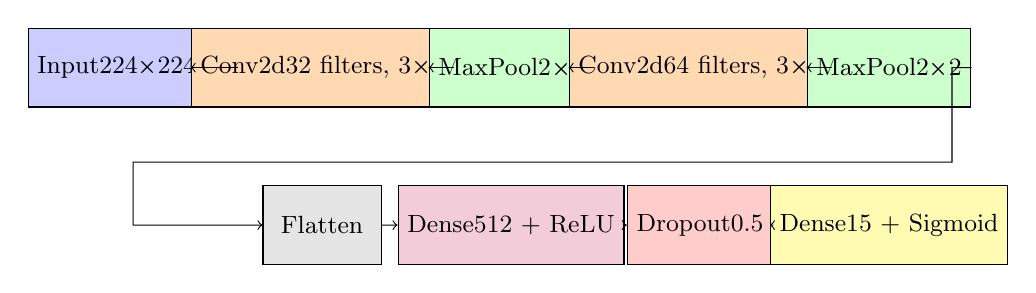
\begin{tikzpicture}[scale=0.8, every node/.style={font=\small}]
    % Input
    \node[draw, fill=blue!20, minimum width=2cm, minimum height=1cm] (input) at (0,0) {Input\\224×224×3};
    
    % Conv1
    \node[draw, fill=orange!30, minimum width=2cm, minimum height=1cm] (conv1) at (3,0) {Conv2d\\32 filters, 3×3};
    
    % Pool1
    \node[draw, fill=green!20, minimum width=1.5cm, minimum height=1cm] (pool1) at (6,0) {MaxPool\\2×2};
    
    % Conv2
    \node[draw, fill=orange!30, minimum width=2cm, minimum height=1cm] (conv2) at (9,0) {Conv2d\\64 filters, 3×3};
    
    % Pool2
    \node[draw, fill=green!20, minimum width=1.5cm, minimum height=1cm] (pool2) at (12,0) {MaxPool\\2×2};
    
    % Flatten
    \node[draw, fill=gray!20, minimum width=1.5cm, minimum height=1cm] (flatten) at (3,-2.5) {Flatten};
    
    % Dense1
    \node[draw, fill=purple!20, minimum width=2cm, minimum height=1cm] (dense1) at (6,-2.5) {Dense\\512 + ReLU};
    
    % Dropout
    \node[draw, fill=red!20, minimum width=1.5cm, minimum height=1cm] (dropout) at (9,-2.5) {Dropout\\0.5};
    
    % Output
    \node[draw, fill=yellow!30, minimum width=2cm, minimum height=1cm] (output) at (12,-2.5) {Dense\\15 + Sigmoid};
    
    % Arrows
    \draw[->] (input) -- (conv1);
    \draw[->] (conv1) -- (pool1);
    \draw[->] (pool1) -- (conv2);
    \draw[->] (conv2) -- (pool2);
    \draw[->] (pool2) -- (13,0) -- (13,-1.5) -- (0,-1.5) -- (0,-2.5) -- (flatten);
    \draw[->] (flatten) -- (dense1);
    \draw[->] (dense1) -- (dropout);
    \draw[->] (dropout) -- (output);
\end{tikzpicture}
\caption{CNN Architecture from paper}
\end{figure}

\section{Mapping Paper → Code}

\coderef{cnn.ipynb}

\subsection{CNN Class Implementation}

\begin{lstlisting}[caption={CNNClassifier in cnn.ipynb (PyTorch)}]
class CNNClassifier(nn.Module):
    def __init__(self, num_classes=15, image_size=224):
        super(CNNClassifier, self).__init__()
        
        # ===== CONVOLUTIONAL LAYERS =====
        # Paper: "convolution layer with 32 3x3 filters"
        self.conv1 = nn.Conv2d(
            in_channels=3,      # RGB input
            out_channels=32,    # 32 filters (from paper)
            kernel_size=3,      # 3x3 kernel (from paper)
            padding=1           # Same padding
        )
        
        # Paper: "max pooling layer with a pool size of 2x2"
        self.pool = nn.MaxPool2d(kernel_size=2, stride=2)
        
        # Paper: "convolution layer with 64 3x3 filters"
        self.conv2 = nn.Conv2d(
            in_channels=32,     # From conv1
            out_channels=64,    # 64 filters (from paper)
            kernel_size=3,      # 3x3 kernel (from paper)
            padding=1
        )
        
        # ===== FULLY CONNECTED LAYERS =====
        # Calculate flatten size after convolutions
        # 224 -> pool -> 112 -> pool -> 56
        # But with valid padding: 224 -> 222 -> 111 -> 109 -> 54
        self.flatten_size = self._get_flatten_size(image_size)
        
        # Paper: "dense layer with 512 units and ReLU activation"
        self.fc1 = nn.Linear(self.flatten_size, 512)
        
        # Paper: "dropout of 0.5"
        self.dropout = nn.Dropout(p=0.5)
        
        # Paper: "output dense layer with 15 units"
        self.fc2 = nn.Linear(512, num_classes)
        
    def _get_flatten_size(self, size):
        """Calculate feature map size after conv layers"""
        # Conv1: (size - 3 + 2*1)/1 + 1 = size (same padding)
        # Pool1: size // 2
        # Conv2: size (same padding)
        # Pool2: size // 2
        size = size // 2  # After pool1
        size = size // 2  # After pool2
        return 64 * size * size  # 64 channels * spatial dims
    
    def forward(self, x):
        # Conv1 + ReLU + Pool
        x = self.pool(F.relu(self.conv1(x)))
        
        # Conv2 + ReLU + Pool
        x = self.pool(F.relu(self.conv2(x)))
        
        # Flatten
        x = x.view(x.size(0), -1)
        
        # FC1 + ReLU + Dropout
        x = self.dropout(F.relu(self.fc1(x)))
        
        # FC2 (no activation - raw logits for BCEWithLogitsLoss)
        x = self.fc2(x)
        
        return x
\end{lstlisting}

\subsection{Detailed Mapping}

\begin{table}[H]
\centering
\caption{Mapping Paper Description → PyTorch Code}
\begin{tabular}{p{5cm}p{5cm}p{3cm}}
\toprule
\textbf{Paper Description} & \textbf{PyTorch Code} & \textbf{Output Shape} \\
\midrule
``convolution layer with 32 3×3 filters'' & \texttt{nn.Conv2d(3, 32, 3, padding=1)} & (B, 32, 224, 224) \\
``max pooling layer 2×2'' & \texttt{nn.MaxPool2d(2, 2)} & (B, 32, 112, 112) \\
``convolution layer with 64 3×3 filters'' & \texttt{nn.Conv2d(32, 64, 3, padding=1)} & (B, 64, 112, 112) \\
``max pooling layer 2×2'' & \texttt{nn.MaxPool2d(2, 2)} & (B, 64, 56, 56) \\
``flatten layer'' & \texttt{x.view(x.size(0), -1)} & (B, 200704) \\
``dense layer with 512 units'' & \texttt{nn.Linear(200704, 512)} & (B, 512) \\
``dropout of 0.5'' & \texttt{nn.Dropout(0.5)} & (B, 512) \\
``output dense layer with 15 units'' & \texttt{nn.Linear(512, 15)} & (B, 15) \\
\bottomrule
\end{tabular}
\end{table}

\section{Detailed Layer Analysis}

\subsection{Layer 1: Conv2d(3, 32, 3)}

\begin{tcolorbox}[colback=blue!5!white,colframe=blue!75!black,title=Analysis: First Convolution Layer]
\textbf{Purpose:} Extract low-level features (edges, gradients, textures)

\textbf{Input:} 224 × 224 × 3 (RGB image)

\textbf{Operation:}
\begin{itemize}
    \item 32 learnable kernels, each 3×3×3
    \item Slide over input with stride 1
    \item With padding=1: output same spatial size
\end{itemize}

\textbf{Parameters:}
\begin{equation}
(3 \times 3 \times 3 + 1) \times 32 = 896 \text{ parameters}
\end{equation}

\textbf{Output:} 224 × 224 × 32
\end{tcolorbox}

\subsection{Layer 2-3: MaxPool → Conv2d(32, 64, 3)}

\begin{tcolorbox}[colback=green!5!white,colframe=green!75!black,title=Analysis: Second Stage]
\textbf{MaxPool2d(2, 2):}
\begin{itemize}
    \item Reduces spatial size: 224 → 112
    \item No learnable parameters
    \item Adds translation invariance
\end{itemize}

\textbf{Conv2d(32, 64, 3):}
\begin{itemize}
    \item Input: 112 × 112 × 32
    \item Learns 64 filters to detect mid-level features
    \item Parameters: $(3 \times 3 \times 32 + 1) \times 64 = 18,496$
    \item Output: 112 × 112 × 64
\end{itemize}
\end{tcolorbox}

\subsection{Flatten + Dense Layers}

\begin{tcolorbox}[colback=purple!5!white,colframe=purple!75!black,title=Analysis: Classification Head]
\textbf{After second pooling:} 56 × 56 × 64 = 200,704 values

\textbf{Dense(200704, 512):}
\begin{itemize}
    \item Largest layer by parameters
    \item Parameters: $200,704 \times 512 + 512 = 102,760,960$
    \item Learns non-local relationships
\end{itemize}

\textbf{Dropout(0.5):}
\begin{itemize}
    \item Randomly zeros 50\% of activations during training
    \item Acts as regularization
    \item No parameters
\end{itemize}

\textbf{Dense(512, 15):}
\begin{itemize}
    \item Output layer for 15 classes
    \item Parameters: $512 \times 15 + 15 = 7,695$
\end{itemize}
\end{tcolorbox}

\section{Total Parameters Analysis}

\begin{table}[H]
\centering
\caption{CNN Parameter Count}
\begin{tabular}{lcr}
\toprule
\textbf{Layer} & \textbf{Formula} & \textbf{Parameters} \\
\midrule
Conv1 & $(3 \times 3 \times 3 + 1) \times 32$ & 896 \\
Conv2 & $(3 \times 3 \times 32 + 1) \times 64$ & 18,496 \\
FC1 & $200,704 \times 512 + 512$ & 102,760,960 \\
FC2 & $512 \times 15 + 15$ & 7,695 \\
\midrule
\textbf{Total} & & \textbf{102,788,047} \\
\bottomrule
\end{tabular}
\end{table}

\begin{tcolorbox}[colback=red!5!white,colframe=red!75!black,title=Observation]
\textbf{99.97\%} of parameters are in the FC1 layer!

This is a common problem with traditional CNNs: the flatten layer creates too many connections.

\textbf{Solutions:}
\begin{itemize}
    \item Global Average Pooling (instead of flatten)
    \item Add more conv layers to reduce spatial size
    \item Use different architecture (ResNet, ViT)
\end{itemize}
\end{tcolorbox}

\section{Loss Function: BCEWithLogitsLoss}

\subsection{Why Not CrossEntropyLoss?}

\begin{table}[H]
\centering
\begin{tabular}{lcc}
\toprule
\textbf{Aspect} & \textbf{CrossEntropyLoss} & \textbf{BCEWithLogitsLoss} \\
\midrule
Task type & Multi-class (one-hot) & Multi-label (independent) \\
Output activation & Softmax & Sigmoid (per class) \\
Sums to 1? & Yes & No \\
NIH dataset & \textcolor{red}{\ding{55}} & \textcolor{green}{\ding{51}} \\
\bottomrule
\end{tabular}
\end{table}

\subsection{BCEWithLogitsLoss Formula}

\begin{equation}
\mathcal{L} = -\frac{1}{N \times C} \sum_{i=1}^{N} \sum_{c=1}^{C} \left[ y_{i,c} \log(\sigma(z_{i,c})) + (1-y_{i,c}) \log(1-\sigma(z_{i,c})) \right]
\end{equation}

Where:
\begin{itemize}
    \item $\sigma(z) = \frac{1}{1 + e^{-z}}$ (sigmoid function)
    \item $y_{i,c} \in \{0, 1\}$ is ground truth
    \item $z_{i,c}$ is raw logit from model
\end{itemize}

\section{Results and Analysis}

\paperref{Section 5 - Experiments}

\subsection{Paper Results}

\begin{tcolorbox}[colback=yellow!5!white,colframe=yellow!75!black,title=Paper Results - CNN]
\begin{itemize}
    \item \textbf{Training Accuracy:} 91\%
    \item \textbf{Validation AUC:} 0.82
    \item \textbf{Test AUC:} 0.82
\end{itemize}
\end{tcolorbox}

\subsection{Performance Analysis}

\begin{tcolorbox}[colback=blue!5!white,colframe=blue!75!black,title=Analysis: Why CNN Performs Worst?]
\textbf{Reasons why CNN has the lowest performance among 5 models:}

\begin{enumerate}
    \item \textbf{Limited Receptive Field:}
    \begin{itemize}
        \item Only 2 conv layers
        \item Small receptive field, hard to capture global features
        \item X-ray pathologies can span the entire image
    \end{itemize}
    
    \item \textbf{No Skip Connections:}
    \begin{itemize}
        \item Gradient must flow through all layers
        \item May suffer from vanishing gradient
        \item Difficult to train deeper variants
    \end{itemize}
    
    \item \textbf{Overfitting Risk:}
    \begin{itemize}
        \item >100M parameters, mostly from FC layer
        \item Dataset of 85K images may not be enough
        \item Despite having dropout 0.5
    \end{itemize}
\end{enumerate}
\end{tcolorbox}

\section{Comparison with Other Architectures}

\begin{table}[H]
\centering
\caption{CNN vs ResNet vs ViT}
\begin{tabular}{lccc}
\toprule
\textbf{Aspect} & \textbf{CNN} & \textbf{ResNet} & \textbf{ViT} \\
\midrule
Depth & 4 layers & 34 layers & 8 blocks \\
Skip connections & No & Yes & No (but attention) \\
Inductive bias & Strong (locality) & Strong & Weak \\
Global context & Poor & Medium & Excellent \\
Parameters & 102M & 21M & 3M \\
Training accuracy & 91\% & 93\% & 93.9\% \\
\bottomrule
\end{tabular}
\end{table}

% ============================================================
% CHAPTER 5: RESNET - RESIDUAL NETWORK
% ============================================================
\chapter{Residual Network (ResNet)}

\section{Motivation: The Degradation Problem}

\subsection{Vấn đề khi training deep networks}

\paperref{Section 3.2 - ResNet}

\begin{tcolorbox}[colback=yellow!5!white,colframe=yellow!75!black,title=Paper Quote - Degradation Problem]
\textit{``However, when we stack many layers to create an extremely deep network, we discover that the training accuracy begins to saturate and then drops off quickly. These observations lead to the understanding of what is commonly referred to as the degradation problem.''}
\end{tcolorbox}

\begin{figure}[H]
\centering
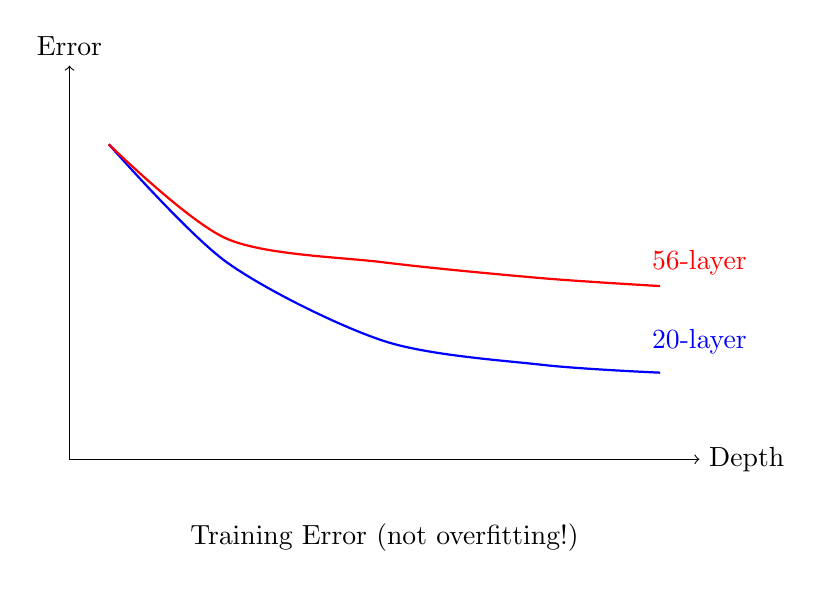
\begin{tikzpicture}
    % Axes
    \draw[->] (0,0) -- (8,0) node[right] {Depth};
    \draw[->] (0,0) -- (0,5) node[above] {Error};
    
    % 20-layer (good)
    \draw[thick, blue] plot[smooth] coordinates {(0.5,4) (2,2.5) (4,1.5) (6,1.2) (7.5,1.1)};
    \node[blue] at (8,1.5) {20-layer};
    
    % 56-layer (bad - degradation)
    \draw[thick, red] plot[smooth] coordinates {(0.5,4) (2,2.8) (4,2.5) (6,2.3) (7.5,2.2)};
    \node[red] at (8,2.5) {56-layer};
    
    \node at (4,-1) {Training Error (not overfitting!)};
\end{tikzpicture}
\caption{Degradation problem: Deeper network có error cao hơn}
\end{figure}

\subsection{Tại sao degradation xảy ra?}

\begin{tcolorbox}[colback=red!5!white,colframe=red!75!black,title=Key Insight]
Degradation \textbf{không phải} do overfitting (training error cũng tăng).

\textbf{Nguyên nhân thực sự:}
\begin{itemize}
    \item Optimization difficulty: Khó tìm được optimal weights
    \item Identity mapping problem: Nếu thêm layer, ít nhất phải learn identity
    \item Nhưng learning identity qua non-linear layers rất khó
\end{itemize}

\textbf{Paradox:} Thêm layer \textit{theo lý thuyết} không thể làm giảm performance (worst case: identity), nhưng thực tế lại giảm!
\end{tcolorbox}

\section{Residual Learning Framework}

\subsection{Ý tưởng cốt lõi}

\paperref{Section 3.2 - ResNet}

\begin{tcolorbox}[colback=yellow!5!white,colframe=yellow!75!black,title=Paper Quote - Skip Connections]
\textit{``To solve the degradation problem, ResNet uses an architecture with residual learning framework called skip connections. Instead of hoping each few stacked layers directly fit a desired underlying mapping, skip connections allow the model to bypass certain layers.''}
\end{tcolorbox}

\subsection{Công thức toán học}

\textbf{Plain Network:}
\begin{equation}
y = F(x)
\end{equation}

\textbf{Residual Network:}
\begin{equation}
y = F(x) + x
\end{equation}

Trong đó:
\begin{itemize}
    \item $x$: Input của block
    \item $F(x)$: Residual function (stacked layers)
    \item $y$: Output = residual + identity
\end{itemize}

\begin{figure}[H]
\centering
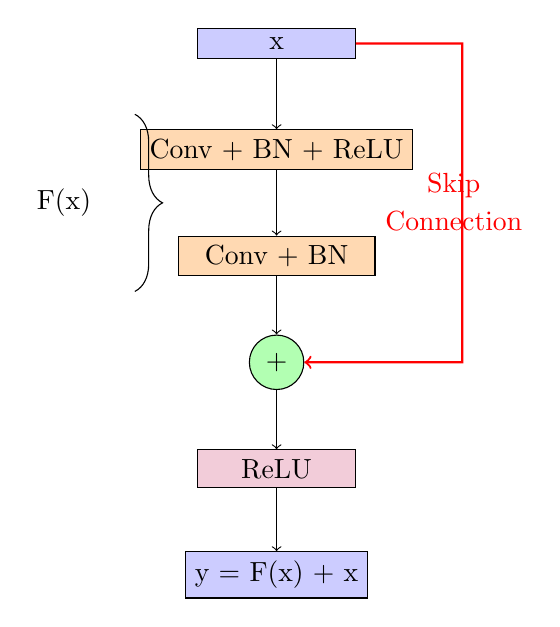
\begin{tikzpicture}[scale=0.9]
    % Input
    \node[draw, fill=blue!20, minimum width=2cm] (input) at (0,0) {x};
    
    % Weight layer 1
    \node[draw, fill=orange!30, minimum width=2.5cm] (w1) at (0,-1.5) {Conv + BN + ReLU};
    
    % Weight layer 2
    \node[draw, fill=orange!30, minimum width=2.5cm] (w2) at (0,-3) {Conv + BN};
    
    % Addition
    \node[draw, circle, fill=green!30] (add) at (0,-4.5) {+};
    
    % ReLU
    \node[draw, fill=purple!20, minimum width=2cm] (relu) at (0,-6) {ReLU};
    
    % Output
    \node[draw, fill=blue!20, minimum width=2cm] (output) at (0,-7.5) {y = F(x) + x};
    
    % Skip connection
    \draw[->] (input) -- (w1);
    \draw[->] (w1) -- (w2);
    \draw[->] (w2) -- (add);
    \draw[->, thick, red] (input.east) -- ++(1.5,0) -- ++(0,-4.5) -- (add.east);
    \node[red] at (2.5,-2) {Skip};
    \node[red] at (2.5,-2.5) {Connection};
    
    \draw[->] (add) -- (relu);
    \draw[->] (relu) -- (output);
    
    % F(x) label
    \draw[decorate, decoration={brace, amplitude=10pt}] (-2,-1) -- (-2,-3.5);
    \node at (-3,-2.25) {F(x)};
\end{tikzpicture}
\caption{Residual Block với Skip Connection}
\end{figure}

\subsection{Tại sao Skip Connection hoạt động?}

\begin{tcolorbox}[colback=green!5!white,colframe=green!75!black,title=Benefits of Skip Connections]
\begin{enumerate}
    \item \textbf{Easy to learn identity:}
    \begin{itemize}
        \item Nếu $F(x) = 0$ → $y = x$ (identity)
        \item Learning $F(x) = 0$ dễ hơn learning complex identity mapping
    \end{itemize}
    
    \item \textbf{Better gradient flow:}
    \begin{itemize}
        \item Gradient có đường tắt qua skip connection
        \item Không bị vanishing qua nhiều layers
    \end{itemize}
    
    \item \textbf{Ensemble effect:}
    \begin{itemize}
        \item ResNet có thể được xem như ensemble của nhiều shallow networks
        \item Skip connections tạo ra exponential paths
    \end{itemize}
\end{enumerate}
\end{tcolorbox}

\subsection{Gradient Flow Analysis}

\begin{equation}
\frac{\partial \mathcal{L}}{\partial x} = \frac{\partial \mathcal{L}}{\partial y} \cdot \frac{\partial y}{\partial x} = \frac{\partial \mathcal{L}}{\partial y} \cdot \left(1 + \frac{\partial F(x)}{\partial x}\right)
\end{equation}

\begin{tcolorbox}[colback=blue!5!white,colframe=blue!75!black,title=Key Observation]
Gradient luôn có thành phần ``1'' từ skip connection.

Ngay cả khi $\frac{\partial F(x)}{\partial x}$ rất nhỏ (vanishing), gradient vẫn flow được!
\end{tcolorbox}

\section{ResNet-34 Architecture}

\paperref{Section 3.2 - ResNet}

\subsection{Paper Description}

\begin{tcolorbox}[colback=yellow!5!white,colframe=yellow!75!black,title=Paper Quote - ResNet Architecture]
\textit{``Similar to VGG-19, ResNet comprises multiple residual blocks, each featuring convolutional layers with 3 × 3 filters. A key difference from the VGG-19 is the presence of skip connections. There are 34 weighted layers in this network, and the input image is 224 × 224.''}
\end{tcolorbox}

\subsection{Chi tiết kiến trúc}

\begin{table}[H]
\centering
\caption{ResNet-34 Architecture}
\begin{tabular}{cccc}
\toprule
\textbf{Stage} & \textbf{Output Size} & \textbf{Layers} & \textbf{Blocks} \\
\midrule
conv1 & 112 × 112 & 7×7 conv, 64, stride 2 & - \\
\midrule
conv2\_x & 56 × 56 & 3×3 max pool, stride 2 & 3 \\
 & & $\begin{bmatrix} 3×3, 64 \\ 3×3, 64 \end{bmatrix}$ & \\
\midrule
conv3\_x & 28 × 28 & $\begin{bmatrix} 3×3, 128 \\ 3×3, 128 \end{bmatrix}$ & 4 \\
\midrule
conv4\_x & 14 × 14 & $\begin{bmatrix} 3×3, 256 \\ 3×3, 256 \end{bmatrix}$ & 6 \\
\midrule
conv5\_x & 7 × 7 & $\begin{bmatrix} 3×3, 512 \\ 3×3, 512 \end{bmatrix}$ & 3 \\
\midrule
 & 1 × 1 & Global Avg Pool, FC 15 & - \\
\bottomrule
\end{tabular}
\end{table}

\textbf{Tổng số layers:} $1 + 2 \times (3 + 4 + 6 + 3) + 1 = 34$ weighted layers

\section{Code Implementation}

\coderef{resnet.ipynb}

\subsection{BasicBlock Class}

\begin{lstlisting}[caption={BasicBlock cho ResNet-18/34}]
class BasicBlock(nn.Module):
    """
    Basic building block for ResNet-18 and ResNet-34.
    Uses two 3x3 convolutions with skip connection.
    """
    expansion = 1  # Output channels = input channels
    
    def __init__(self, in_channels, out_channels, stride=1, downsample=None):
        super(BasicBlock, self).__init__()
        
        # ===== First conv layer =====
        # Paper: "3x3 convolution"
        self.conv1 = nn.Conv2d(
            in_channels, out_channels,
            kernel_size=3,
            stride=stride,      # stride=2 for downsampling
            padding=1,
            bias=False          # BN handles bias
        )
        self.bn1 = nn.BatchNorm2d(out_channels)
        
        # ===== Second conv layer =====
        self.conv2 = nn.Conv2d(
            out_channels, out_channels,
            kernel_size=3,
            stride=1,
            padding=1,
            bias=False
        )
        self.bn2 = nn.BatchNorm2d(out_channels)
        
        # ===== Skip connection =====
        # If dimensions change, need 1x1 conv to match
        self.downsample = downsample
        self.stride = stride
        
    def forward(self, x):
        identity = x  # Save for skip connection
        
        # Main path: conv -> bn -> relu -> conv -> bn
        out = self.conv1(x)
        out = self.bn1(out)
        out = F.relu(out)
        
        out = self.conv2(out)
        out = self.bn2(out)
        
        # Skip connection (match dimensions if needed)
        if self.downsample is not None:
            identity = self.downsample(x)
        
        # Add skip connection
        out += identity  # y = F(x) + x
        out = F.relu(out)  # Final activation
        
        return out
\end{lstlisting}

\subsection{ResNet Main Class}

\begin{lstlisting}[caption={ResNet-34 main class}]
class ResNet(nn.Module):
    def __init__(self, block, layers, num_classes=15):
        """
        Args:
            block: BasicBlock (for ResNet-18/34) or Bottleneck (for 50/101/152)
            layers: [3, 4, 6, 3] for ResNet-34
            num_classes: 15 for chest x-ray
        """
        super(ResNet, self).__init__()
        self.in_channels = 64
        
        # ===== Initial Convolution =====
        # Paper: "7x7 conv, 64, stride 2"
        self.conv1 = nn.Conv2d(
            3, 64, 
            kernel_size=7, 
            stride=2, 
            padding=3,
            bias=False
        )
        self.bn1 = nn.BatchNorm2d(64)
        self.relu = nn.ReLU(inplace=True)
        
        # Paper: "3x3 max pool, stride 2"
        self.maxpool = nn.MaxPool2d(kernel_size=3, stride=2, padding=1)
        
        # ===== Residual Stages =====
        # layers = [3, 4, 6, 3] for ResNet-34
        self.layer1 = self._make_layer(block, 64, layers[0])       # 3 blocks
        self.layer2 = self._make_layer(block, 128, layers[1], stride=2)  # 4 blocks
        self.layer3 = self._make_layer(block, 256, layers[2], stride=2)  # 6 blocks
        self.layer4 = self._make_layer(block, 512, layers[3], stride=2)  # 3 blocks
        
        # ===== Global Average Pooling =====
        self.avgpool = nn.AdaptiveAvgPool2d((1, 1))
        
        # ===== Classification Head =====
        self.fc = nn.Linear(512 * block.expansion, num_classes)
        
        # ===== Weight Initialization =====
        self._initialize_weights()
        
    def _make_layer(self, block, out_channels, blocks, stride=1):
        """Create a stage with multiple residual blocks."""
        downsample = None
        
        # If spatial size or channels change, need projection
        if stride != 1 or self.in_channels != out_channels * block.expansion:
            downsample = nn.Sequential(
                nn.Conv2d(
                    self.in_channels,
                    out_channels * block.expansion,
                    kernel_size=1,
                    stride=stride,
                    bias=False
                ),
                nn.BatchNorm2d(out_channels * block.expansion)
            )
        
        layers = []
        # First block may have stride > 1 (downsampling)
        layers.append(block(self.in_channels, out_channels, stride, downsample))
        self.in_channels = out_channels * block.expansion
        
        # Remaining blocks have stride = 1
        for _ in range(1, blocks):
            layers.append(block(self.in_channels, out_channels))
        
        return nn.Sequential(*layers)
    
    def _initialize_weights(self):
        """Kaiming initialization for conv layers."""
        for m in self.modules():
            if isinstance(m, nn.Conv2d):
                nn.init.kaiming_normal_(
                    m.weight, mode='fan_out', nonlinearity='relu'
                )
            elif isinstance(m, nn.BatchNorm2d):
                nn.init.constant_(m.weight, 1)
                nn.init.constant_(m.bias, 0)
    
    def forward(self, x):
        # Initial: 224x224x3 -> 112x112x64 -> 56x56x64
        x = self.conv1(x)      # 224 -> 112
        x = self.bn1(x)
        x = self.relu(x)
        x = self.maxpool(x)    # 112 -> 56
        
        # Residual stages
        x = self.layer1(x)     # 56x56x64
        x = self.layer2(x)     # 28x28x128
        x = self.layer3(x)     # 14x14x256
        x = self.layer4(x)     # 7x7x512
        
        # Global average pooling + FC
        x = self.avgpool(x)    # 1x1x512
        x = torch.flatten(x, 1)
        x = self.fc(x)         # 15 classes
        
        return x
\end{lstlisting}

\subsection{Model Instantiation}

\begin{lstlisting}[caption={Tạo ResNet-34 instance}]
def resnet34(num_classes=15):
    """Create ResNet-34 model."""
    return ResNet(
        block=BasicBlock,
        layers=[3, 4, 6, 3],  # ResNet-34 configuration
        num_classes=num_classes
    )

# Usage
model = resnet34(num_classes=15)
\end{lstlisting}

\section{Detailed Mapping: Paper → Code}

\begin{table}[H]
\centering
\caption{ResNet-34: Paper → Code Mapping}
\begin{tabular}{p{4cm}p{5cm}p{4cm}}
\toprule
\textbf{Paper Description} & \textbf{PyTorch Code} & \textbf{Output} \\
\midrule
``34 weighted layers'' & \texttt{layers=[3,4,6,3]} → $2 \times 16 + 2 = 34$ & - \\
``7×7 conv, stride 2'' & \texttt{nn.Conv2d(3,64,7,stride=2,padding=3)} & 112×112×64 \\
``3×3 max pool'' & \texttt{nn.MaxPool2d(3,stride=2,padding=1)} & 56×56×64 \\
``skip connections'' & \texttt{out += identity} & - \\
``3×3 filters'' & \texttt{kernel\_size=3} trong BasicBlock & - \\
\bottomrule
\end{tabular}
\end{table}

\section{Batch Normalization}

\subsection{Công thức}

\begin{equation}
\hat{x}_i = \frac{x_i - \mu_B}{\sqrt{\sigma_B^2 + \epsilon}}
\end{equation}
\begin{equation}
y_i = \gamma \hat{x}_i + \beta
\end{equation}

Trong đó:
\begin{itemize}
    \item $\mu_B, \sigma_B^2$: Mean và variance của mini-batch
    \item $\gamma, \beta$: Learnable scale và shift
    \item $\epsilon$: Small constant for numerical stability
\end{itemize}

\subsection{Tại sao BatchNorm quan trọng với ResNet?}

\begin{tcolorbox}[colback=blue!5!white,colframe=blue!75!black,title=BatchNorm Benefits]
\begin{enumerate}
    \item \textbf{Internal Covariate Shift:} Normalize activations giúp training stable
    \item \textbf{Higher Learning Rate:} Có thể dùng LR cao hơn
    \item \textbf{Regularization Effect:} Giảm overfitting (nhẹ)
    \item \textbf{ResNet Specific:} BN trước skip connection giúp gradient flow tốt hơn
\end{enumerate}
\end{tcolorbox}

\section{Global Average Pooling vs Flatten}

\subsection{So sánh}

\begin{table}[H]
\centering
\caption{Global Average Pooling vs Flatten}
\begin{tabular}{lcc}
\toprule
\textbf{Aspect} & \textbf{Flatten (CNN)} & \textbf{GAP (ResNet)} \\
\midrule
Output size & $H \times W \times C$ & $C$ \\
Parameters in FC & Very large & Small \\
Overfitting risk & High & Low \\
Spatial info & Preserved & Lost (averaged) \\
Translation invariance & No & Yes \\
\bottomrule
\end{tabular}
\end{table}

\subsection{Ví dụ cụ thể}

\begin{lstlisting}[caption={GAP vs Flatten comparison}]
# After conv layers: feature map is 7x7x512

# Option 1: Flatten (like CNN)
flatten_output = 7 * 7 * 512  # = 25,088
fc_params = 25088 * 15 + 15   # = 376,335 parameters

# Option 2: Global Average Pooling (like ResNet)
gap_output = 512  # Average over 7x7 spatial dims
fc_params = 512 * 15 + 15     # = 7,695 parameters

# GAP giảm 98% parameters trong FC layer!
\end{lstlisting}

\section{Parameter Count Analysis}

\begin{table}[H]
\centering
\caption{ResNet-34 Parameter Breakdown}
\begin{tabular}{lcrr}
\toprule
\textbf{Stage} & \textbf{Blocks} & \textbf{Channels} & \textbf{Params} \\
\midrule
conv1 & 1 & 3 → 64 & 9,408 \\
layer1 & 3 & 64 → 64 & 221,184 \\
layer2 & 4 & 64 → 128 & 1,114,624 \\
layer3 & 6 & 128 → 256 & 6,818,304 \\
layer4 & 3 & 256 → 512 & 13,631,488 \\
FC & 1 & 512 → 15 & 7,695 \\
\midrule
\textbf{Total} & & & \textbf{21,802,703} \\
\bottomrule
\end{tabular}
\end{table}

\textbf{So sánh:} ResNet-34 có \textbf{21M params} vs CNN có \textbf{102M params}, nhưng sâu hơn (34 layers vs 4 layers) và hiệu quả hơn!

\section{Results Analysis}

\paperref{Section 5 - Experiments}

\subsection{Paper Results}

\begin{tcolorbox}[colback=yellow!5!white,colframe=yellow!75!black,title=Paper Results - ResNet]
\begin{itemize}
    \item \textbf{Training Accuracy:} 93\%
    \item \textbf{Validation AUC:} 0.86
    \item \textbf{Test AUC:} 0.86
\end{itemize}
\end{tcolorbox}

\subsection{So sánh với CNN}

\begin{table}[H]
\centering
\caption{CNN vs ResNet Performance}
\begin{tabular}{lcc}
\toprule
\textbf{Metric} & \textbf{CNN} & \textbf{ResNet-34} \\
\midrule
Training Accuracy & 91\% & 93\% (+2\%) \\
Test AUC & 0.82 & 0.86 (+0.04) \\
Parameters & 102M & 21M \\
Depth & 4 layers & 34 layers \\
\bottomrule
\end{tabular}
\end{table}

\subsection{Tại sao ResNet tốt hơn?}

\begin{tcolorbox}[colback=green!5!white,colframe=green!75!black,title=Analysis: ResNet Advantages]
\begin{enumerate}
    \item \textbf{Deeper Feature Hierarchy:}
    \begin{itemize}
        \item 34 layers vs 4 layers
        \item Có thể learn complex hierarchical features
        \item X-ray patterns có nhiều levels of abstraction
    \end{itemize}
    
    \item \textbf{Better Gradient Flow:}
    \begin{itemize}
        \item Skip connections cho phép gradient flow trực tiếp
        \item Training stable hơn
    \end{itemize}
    
    \item \textbf{Efficient Parameter Usage:}
    \begin{itemize}
        \item GAP thay vì flatten
        \item Ít parameters hơn nhưng more expressive
    \end{itemize}
    
    \item \textbf{Better Regularization:}
    \begin{itemize}
        \item Batch Normalization trong mọi block
        \item Weight decay hiệu quả hơn
    \end{itemize}
\end{enumerate}
\end{tcolorbox}

% ============================================================
% CHAPTER 6: VISION TRANSFORMER (ViT)
% Deep Expert Analysis - Main Focus Chapter
% ============================================================
\chapter{Vision Transformer (ViT)}

\section{Motivation: From NLP to Vision}

\subsection{The Transformer Revolution}

\begin{tcolorbox}[colback=blue!5!white,colframe=blue!75!black,title=Historical Context]
\textbf{2017:} ``Attention Is All You Need'' (Vaswani et al.)
\begin{itemize}
    \item Transformer thay thế RNN trong NLP
    \item Self-attention captures long-range dependencies
    \item Parallelizable → faster training
\end{itemize}

\textbf{2020:} ``An Image is Worth 16×16 Words'' (Dosovitskiy et al.)
\begin{itemize}
    \item Áp dụng Transformer pure cho vision
    \item Images = sequences of patches
    \item State-of-the-art khi pretrained on large data
\end{itemize}
\end{tcolorbox}

\subsection{Paper Motivation}

\paperref{Section 3.3 - Vision Transformer}

\begin{tcolorbox}[colback=yellow!5!white,colframe=yellow!75!black,title=Paper Quote - ViT Motivation]
\textit{``Vision Transformer (ViT) [3] follows an approach to image classification by treating an image as a sequence of patches and processing it using a standard Transformer encoder like the ones used in NLP.''}
\end{tcolorbox}

\subsection{CNN vs Transformer Inductive Biases}

\begin{table}[H]
\centering
\caption{Inductive Biases: CNN vs ViT}
\begin{tabular}{lcc}
\toprule
\textbf{Inductive Bias} & \textbf{CNN} & \textbf{ViT} \\
\midrule
Locality & \checkmark Strong & \texttimes Weak \\
Translation Equivariance & \checkmark Built-in & \texttimes Learned \\
2D Structure & \checkmark Preserved & \texttimes Flattened \\
Long-range Dependencies & \texttimes Limited & \checkmark Global \\
Data Efficiency & \checkmark Good & \texttimes Needs more data \\
Scalability & Limited & \checkmark Scales well \\
\bottomrule
\end{tabular}
\end{table}

\section{ViT Architecture Overview}

\begin{figure}[H]
\centering
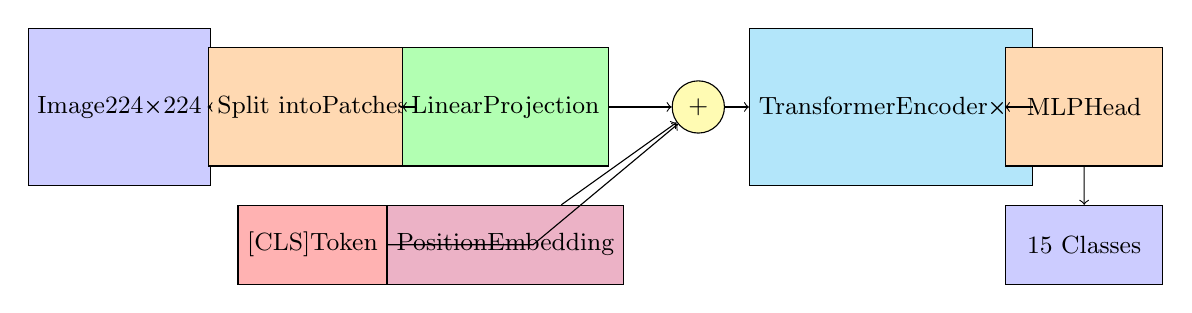
\begin{tikzpicture}[scale=0.7, every node/.style={font=\small}]
    % Input image
    \node[draw, fill=blue!20, minimum width=2cm, minimum height=2cm] (img) at (0,0) {Image\\224×224};
    
    % Patches
    \node[draw, fill=orange!30, minimum width=2cm, minimum height=1.5cm] (patch) at (3.5,0) {Split into\\Patches};
    
    % Linear projection
    \node[draw, fill=green!30, minimum width=2cm, minimum height=1.5cm] (proj) at (7,0) {Linear\\Projection};
    
    % Position embedding
    \node[draw, fill=purple!30, minimum width=2cm, minimum height=1cm] (pos) at (7,-2.5) {Position\\Embedding};
    
    % CLS token
    \node[draw, fill=red!30, minimum width=1.5cm, minimum height=1cm] (cls) at (3.5,-2.5) {[CLS]\\Token};
    
    % Add
    \node[draw, circle, fill=yellow!30] (add) at (10.5,0) {+};
    
    % Transformer Encoder
    \node[draw, fill=cyan!30, minimum width=2.5cm, minimum height=2cm] (trans) at (14,0) {Transformer\\Encoder\\×L};
    
    % MLP Head
    \node[draw, fill=orange!30, minimum width=2cm, minimum height=1.5cm] (mlp) at (17.5,0) {MLP\\Head};
    
    % Output
    \node[draw, fill=blue!20, minimum width=2cm, minimum height=1cm] (out) at (17.5,-2.5) {15 Classes};
    
    % Arrows
    \draw[->] (img) -- (patch);
    \draw[->] (patch) -- (proj);
    \draw[->] (proj) -- (add);
    \draw[->] (pos) -- (add);
    \draw[->] (cls) -- ++(4,0) -- (add);
    \draw[->] (add) -- (trans);
    \draw[->] (trans) -- (mlp);
    \draw[->] (mlp) -- (out);
\end{tikzpicture}
\caption{Vision Transformer Architecture Overview}
\end{figure}

\section{Step 1: Patch Embedding}

\subsection{Concept}

\paperref{Section 3.3 - Vision Transformer}

\begin{tcolorbox}[colback=yellow!5!white,colframe=yellow!75!black,title=Paper Quote - Patch Embedding]
\textit{``This involves dividing the image into fixed-size non-overlapping patches, which are then linearly embedded. In our experiments, we fix a patch size of 32 × 32 for all our Vision Transformer models.''}
\end{tcolorbox}

\subsection{Toán học}

Với image $x \in \mathbb{R}^{H \times W \times C}$ và patch size $P$:

\textbf{Step 1: Chia patch}
\begin{equation}
\text{Number of patches: } N = \frac{H \times W}{P^2} = \frac{224 \times 224}{32 \times 32} = 49
\end{equation}

\textbf{Step 2: Flatten mỗi patch}
\begin{equation}
x_p^i \in \mathbb{R}^{P^2 \cdot C} = \mathbb{R}^{32 \times 32 \times 3} = \mathbb{R}^{3072}
\end{equation}

\textbf{Step 3: Linear projection}
\begin{equation}
z_0^i = x_p^i \cdot E + b, \quad E \in \mathbb{R}^{(P^2 \cdot C) \times D}
\end{equation}

Trong đó $D$ là embedding dimension (projection\_dim = 64 trong paper).

\subsection{Implementation trong Code}

\coderef{ViT-v1.ipynb}

\begin{lstlisting}[caption={PatchEmbedding Class - Phiên bản 1}]
class PatchEmbedding(nn.Module):
    """
    Convert image into patch embeddings.
    
    Paper: "dividing the image into fixed-size non-overlapping patches"
    Implementation: Use Conv2d with kernel_size=stride=patch_size
    """
    def __init__(self, img_size=224, patch_size=32, in_channels=3, embed_dim=64):
        super(PatchEmbedding, self).__init__()
        self.img_size = img_size
        self.patch_size = patch_size
        self.num_patches = (img_size // patch_size) ** 2  # 49 patches
        
        # ===== Linear Projection via Conv2d =====
        # Equivalent to: flatten patch -> linear layer
        # But more efficient implementation
        self.projection = nn.Conv2d(
            in_channels=in_channels,   # 3 (RGB)
            out_channels=embed_dim,    # 64 (projection_dim)
            kernel_size=patch_size,    # 32x32
            stride=patch_size          # Non-overlapping
        )
        
    def forward(self, x):
        # x: (B, 3, 224, 224)
        
        # Apply projection
        x = self.projection(x)
        # Shape: (B, embed_dim, num_patches_h, num_patches_w)
        # = (B, 64, 7, 7)
        
        # Flatten spatial dimensions
        x = x.flatten(2)
        # Shape: (B, 64, 49)
        
        # Transpose to (B, num_patches, embed_dim)
        x = x.transpose(1, 2)
        # Shape: (B, 49, 64)
        
        return x
\end{lstlisting}

\subsection{Tại sao dùng Conv2d cho Linear Projection?}

\begin{tcolorbox}[colback=green!5!white,colframe=green!75!black,title=Conv2d = Efficient Linear Projection]
\textbf{Method 1: Naive (unfold + linear)}
\begin{lstlisting}[style=plain]
patches = x.unfold(2, P, P).unfold(3, P, P)  # Extract patches
patches = patches.reshape(B, N, P*P*C)       # Flatten
embeddings = linear(patches)                  # Project
\end{lstlisting}

\textbf{Method 2: Conv2d (elegant)}
\begin{lstlisting}[style=plain]
embeddings = conv2d(x, kernel=P, stride=P)   # One operation!
\end{lstlisting}

\textbf{Equivalence:} Conv2d với kernel\_size=stride=P chính là:
\begin{itemize}
    \item Extract non-overlapping patches
    \item Apply same linear transformation to each patch
    \item Output: one value per patch per filter = embedding
\end{itemize}
\end{tcolorbox}

\section{Step 2: Positional Embedding}

\subsection{Tại sao cần Position Information?}

\begin{tcolorbox}[colback=red!5!white,colframe=red!75!black,title=Problem: Self-Attention is Permutation Invariant]
Self-attention treats input as a \textbf{set}, not a \textbf{sequence}.

\textbf{Ví dụ:} Với patches $[p_1, p_2, p_3]$:
\begin{itemize}
    \item Attention($[p_1, p_2, p_3]$) = Attention($[p_3, p_1, p_2]$)
    \item Model không biết patch nào ở đâu!
    \item Vị trí quan trọng: lung ở giữa, heart ở trái
\end{itemize}

\textbf{Solution:} Add positional information to embeddings.
\end{tcolorbox}

\subsection{Learnable vs Fixed Positional Embedding}

\begin{table}[H]
\centering
\caption{Positional Embedding Types}
\begin{tabular}{lp{5cm}p{5cm}}
\toprule
\textbf{Type} & \textbf{Sinusoidal (Fixed)} & \textbf{Learnable} \\
\midrule
Formula & $PE_{pos,2i} = \sin(pos/10000^{2i/d})$ & Random init, trained \\
Parameters & 0 & $N \times D$ \\
Generalization & To any length & Fixed length \\
ViT choice & - & \checkmark Used \\
\bottomrule
\end{tabular}
\end{table}

\subsection{Implementation}

\begin{lstlisting}[caption={Positional Embedding trong ViT}]
class VisionTransformer(nn.Module):
    def __init__(self, ...):
        # ...
        
        # ===== Positional Embedding =====
        # Paper: "learnable 1D position embeddings"
        # Shape: (1, num_patches + 1, embed_dim) = (1, 50, 64)
        # +1 for CLS token
        self.pos_embedding = nn.Parameter(
            torch.randn(1, num_patches + 1, embed_dim)
        )
        
    def forward(self, x):
        # After patch embedding: (B, 49, 64)
        
        # Add CLS token
        cls_tokens = self.cls_token.expand(B, -1, -1)  # (B, 1, 64)
        x = torch.cat([cls_tokens, x], dim=1)          # (B, 50, 64)
        
        # Add positional embedding
        x = x + self.pos_embedding  # (B, 50, 64) + (1, 50, 64) broadcast
        
        return x
\end{lstlisting}

\section{Step 3: [CLS] Token}

\subsection{Origin: BERT}

\begin{tcolorbox}[colback=blue!5!white,colframe=blue!75!black,title=CLS Token Concept]
\textbf{Nguồn gốc:} BERT (NLP)
\begin{itemize}
    \item Special token prepended to input sequence
    \item Learns to aggregate information from all tokens
    \item Used for classification tasks
\end{itemize}

\textbf{Trong ViT:}
\begin{itemize}
    \item Prepend một learnable token trước patch embeddings
    \item Sau Transformer: CLS token ``nhìn'' toàn bộ image
    \item Dùng CLS token cho final classification
\end{itemize}
\end{tcolorbox}

\subsection{Implementation}

\begin{lstlisting}[caption={CLS Token Implementation}]
class VisionTransformer(nn.Module):
    def __init__(self, ...):
        # ===== CLS Token =====
        # Learnable parameter
        # Shape: (1, 1, embed_dim) = (1, 1, 64)
        self.cls_token = nn.Parameter(
            torch.zeros(1, 1, embed_dim)
        )
        
    def forward(self, x):
        B = x.shape[0]
        
        # Patch embedding: (B, 49, 64)
        x = self.patch_embed(x)
        
        # Expand CLS token for batch
        cls_tokens = self.cls_token.expand(B, -1, -1)  # (B, 1, 64)
        
        # Concatenate: CLS + patches
        x = torch.cat([cls_tokens, x], dim=1)  # (B, 50, 64)
        # Position 0 = CLS, Positions 1-49 = patches
        
        # After Transformer encoder...
        x = self.transformer(x)  # (B, 50, 64)
        
        # Extract CLS token for classification
        cls_output = x[:, 0]  # (B, 64) - first token
        
        return self.head(cls_output)
\end{lstlisting}

\section{Step 4: Transformer Encoder}

\subsection{Self-Attention Mechanism}

\paperref{Section 3.3 - Vision Transformer}

\begin{tcolorbox}[colback=yellow!5!white,colframe=yellow!75!black,title=Paper Quote - Multi-Head Attention]
\textit{``Our Vision Transformer implementation includes Multi-Head Self-Attention (MHSA). It also includes MLP blocks and Layer Normalization (LN) applied before every block, and residual connections applied after every block.''}
\end{tcolorbox}

\subsubsection{Single-Head Attention}

\begin{equation}
\text{Attention}(Q, K, V) = \text{softmax}\left(\frac{QK^T}{\sqrt{d_k}}\right) V
\end{equation}

Trong đó:
\begin{itemize}
    \item $Q = XW^Q$ (Queries): ``What am I looking for?''
    \item $K = XW^K$ (Keys): ``What do I contain?''
    \item $V = XW^V$ (Values): ``What information do I provide?''
    \item $\sqrt{d_k}$: Scaling factor để ổn định gradient
\end{itemize}

\begin{figure}[H]
\centering
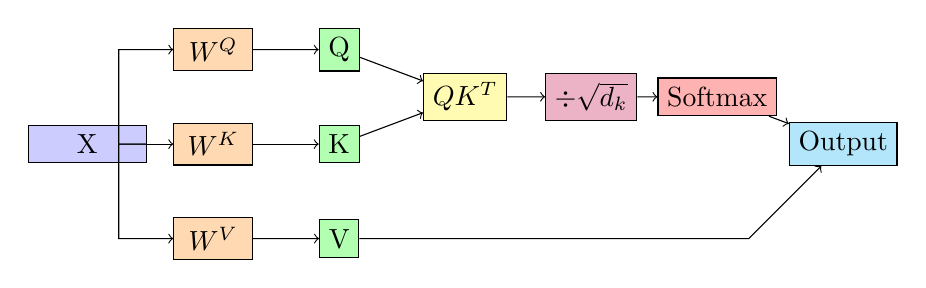
\begin{tikzpicture}[scale=0.8]
    % Input
    \node[draw, fill=blue!20, minimum width=1.5cm] (x) at (0,0) {X};
    
    % Q, K, V projections
    \node[draw, fill=orange!30, minimum width=1cm] (wq) at (2,1.5) {$W^Q$};
    \node[draw, fill=orange!30, minimum width=1cm] (wk) at (2,0) {$W^K$};
    \node[draw, fill=orange!30, minimum width=1cm] (wv) at (2,-1.5) {$W^V$};
    
    % Q, K, V
    \node[draw, fill=green!30] (q) at (4,1.5) {Q};
    \node[draw, fill=green!30] (k) at (4,0) {K};
    \node[draw, fill=green!30] (v) at (4,-1.5) {V};
    
    % MatMul QK
    \node[draw, fill=yellow!30] (qk) at (6,0.75) {$QK^T$};
    
    % Scale
    \node[draw, fill=purple!30] (scale) at (8,0.75) {$\div\sqrt{d_k}$};
    
    % Softmax
    \node[draw, fill=red!30] (soft) at (10,0.75) {Softmax};
    
    % MatMul with V
    \node[draw, fill=cyan!30] (out) at (12,0) {Output};
    
    % Arrows
    \draw[->] (x) -- ++(0.5,0) -- ++(0,1.5) -- (wq);
    \draw[->] (x) -- (wk);
    \draw[->] (x) -- ++(0.5,0) -- ++(0,-1.5) -- (wv);
    
    \draw[->] (wq) -- (q);
    \draw[->] (wk) -- (k);
    \draw[->] (wv) -- (v);
    
    \draw[->] (q) -- (qk);
    \draw[->] (k) -- (qk);
    \draw[->] (qk) -- (scale);
    \draw[->] (scale) -- (soft);
    \draw[->] (soft) -- (out);
    \draw[->] (v) -- ++(6.5,0) -- (out);
\end{tikzpicture}
\caption{Scaled Dot-Product Attention}
\end{figure}

\subsubsection{Multi-Head Attention}

\begin{equation}
\text{MultiHead}(Q, K, V) = \text{Concat}(\text{head}_1, ..., \text{head}_h) W^O
\end{equation}

\begin{equation}
\text{head}_i = \text{Attention}(QW_i^Q, KW_i^K, VW_i^V)
\end{equation}

\begin{tcolorbox}[colback=green!5!white,colframe=green!75!black,title=Why Multi-Head?]
\begin{itemize}
    \item Mỗi head có thể attend to different aspects
    \item Head 1: positional relationships
    \item Head 2: color similarities
    \item Head 3: shape patterns
    \item Concatenate → richer representation
\end{itemize}
\end{tcolorbox}

\subsection{Implementation}

\coderef{ViT-v1.ipynb}

\begin{lstlisting}[caption={TransformerEncoderBlock Implementation}]
class TransformerEncoderBlock(nn.Module):
    """
    Single Transformer Encoder block.
    
    Architecture:
        x -> LayerNorm -> MHSA -> + -> LayerNorm -> MLP -> + -> output
             |__________________|      |_______________|
                 Skip connection          Skip connection
    """
    def __init__(self, embed_dim, num_heads, mlp_ratio=4.0, dropout=0.1):
        super(TransformerEncoderBlock, self).__init__()
        
        # ===== Layer Normalization (Pre-Norm) =====
        # Paper: "Layer Normalization applied before every block"
        self.norm1 = nn.LayerNorm(embed_dim)
        self.norm2 = nn.LayerNorm(embed_dim)
        
        # ===== Multi-Head Self-Attention =====
        # Paper: "Multi-Head Self-Attention (MHSA)"
        self.attn = nn.MultiheadAttention(
            embed_dim=embed_dim,   # 64
            num_heads=num_heads,   # 4 heads -> head_dim = 16
            dropout=dropout,
            batch_first=True       # Input: (B, N, D)
        )
        
        # ===== MLP Block =====
        # Paper: "MLP blocks"
        mlp_hidden_dim = int(embed_dim * mlp_ratio)  # 64 * 4 = 256
        self.mlp = MLP(
            in_features=embed_dim,
            hidden_features=mlp_hidden_dim,
            out_features=embed_dim,
            dropout=dropout
        )
        
        self.dropout = nn.Dropout(dropout)
        
    def forward(self, x):
        # ===== Attention Block with Skip Connection =====
        # Pre-LayerNorm (ViT uses pre-norm, not post-norm)
        attn_input = self.norm1(x)
        
        # Multi-Head Self-Attention
        # Query = Key = Value = same input (self-attention)
        attn_output, _ = self.attn(
            query=attn_input,
            key=attn_input,
            value=attn_input
        )
        
        # Skip connection (residual)
        x = x + self.dropout(attn_output)
        
        # ===== MLP Block with Skip Connection =====
        mlp_input = self.norm2(x)
        mlp_output = self.mlp(mlp_input)
        
        # Skip connection
        x = x + self.dropout(mlp_output)
        
        return x
\end{lstlisting}

\subsection{MLP Block}

\begin{lstlisting}[caption={MLP Block (Feed-Forward Network)}]
class MLP(nn.Module):
    """
    MLP block in Transformer.
    
    Architecture: Linear -> GELU -> Dropout -> Linear -> Dropout
    """
    def __init__(self, in_features, hidden_features, out_features, dropout=0.1):
        super(MLP, self).__init__()
        
        self.fc1 = nn.Linear(in_features, hidden_features)  # 64 -> 256
        self.act = nn.GELU()  # Gaussian Error Linear Unit
        self.fc2 = nn.Linear(hidden_features, out_features)  # 256 -> 64
        self.dropout = nn.Dropout(dropout)
        
    def forward(self, x):
        x = self.fc1(x)
        x = self.act(x)
        x = self.dropout(x)
        x = self.fc2(x)
        x = self.dropout(x)
        return x
\end{lstlisting}

\subsubsection{GELU Activation}

\begin{equation}
\text{GELU}(x) = x \cdot \Phi(x) = x \cdot \frac{1}{2}\left[1 + \text{erf}\left(\frac{x}{\sqrt{2}}\right)\right]
\end{equation}

\begin{tcolorbox}[colback=blue!5!white,colframe=blue!75!black,title=GELU vs ReLU]
\begin{itemize}
    \item GELU: Smooth approximation of ReLU
    \item Có curvature tại 0 (không có kink như ReLU)
    \item Cho phép small negative values
    \item Standard trong Transformers (BERT, GPT, ViT)
\end{itemize}
\end{tcolorbox}

\section{Complete ViT Implementation}

\begin{lstlisting}[caption={Complete VisionTransformer Class}]
class VisionTransformer(nn.Module):
    """
    Vision Transformer for Chest X-ray Classification.
    
    Paper configuration:
        - patch_size: 32 (ViT-v1/32)
        - embed_dim: 64
        - depth: 8 transformer blocks
        - num_heads: 4
        - mlp_ratio: 4.0
        - num_classes: 15
    """
    def __init__(
        self,
        img_size=224,
        patch_size=32,
        in_channels=3,
        num_classes=15,
        embed_dim=64,
        depth=8,
        num_heads=4,
        mlp_ratio=4.0,
        dropout=0.1
    ):
        super(VisionTransformer, self).__init__()
        
        # ===== Patch Embedding =====
        self.patch_embed = PatchEmbedding(
            img_size=img_size,
            patch_size=patch_size,
            in_channels=in_channels,
            embed_dim=embed_dim
        )
        num_patches = self.patch_embed.num_patches  # 49
        
        # ===== CLS Token =====
        self.cls_token = nn.Parameter(torch.zeros(1, 1, embed_dim))
        
        # ===== Positional Embedding =====
        # +1 for CLS token
        self.pos_embedding = nn.Parameter(
            torch.randn(1, num_patches + 1, embed_dim) * 0.02
        )
        
        self.pos_dropout = nn.Dropout(dropout)
        
        # ===== Transformer Encoder =====
        self.transformer = nn.Sequential(*[
            TransformerEncoderBlock(
                embed_dim=embed_dim,
                num_heads=num_heads,
                mlp_ratio=mlp_ratio,
                dropout=dropout
            )
            for _ in range(depth)  # 8 blocks
        ])
        
        # ===== Final LayerNorm =====
        self.norm = nn.LayerNorm(embed_dim)
        
        # ===== Classification Head =====
        self.head = nn.Linear(embed_dim, num_classes)
        
        # ===== Weight Initialization =====
        self._init_weights()
        
    def _init_weights(self):
        # Initialize cls_token
        nn.init.normal_(self.cls_token, std=0.02)
        
        # Initialize linear layers
        for m in self.modules():
            if isinstance(m, nn.Linear):
                nn.init.xavier_uniform_(m.weight)
                if m.bias is not None:
                    nn.init.zeros_(m.bias)
        
    def forward(self, x):
        B = x.shape[0]
        
        # 1. Patch Embedding: (B, 3, 224, 224) -> (B, 49, 64)
        x = self.patch_embed(x)
        
        # 2. Prepend CLS Token: (B, 49, 64) -> (B, 50, 64)
        cls_tokens = self.cls_token.expand(B, -1, -1)
        x = torch.cat([cls_tokens, x], dim=1)
        
        # 3. Add Positional Embedding
        x = x + self.pos_embedding
        x = self.pos_dropout(x)
        
        # 4. Transformer Encoder: (B, 50, 64) -> (B, 50, 64)
        x = self.transformer(x)
        
        # 5. Final Norm
        x = self.norm(x)
        
        # 6. Extract CLS Token: (B, 50, 64) -> (B, 64)
        cls_output = x[:, 0]
        
        # 7. Classification Head: (B, 64) -> (B, 15)
        output = self.head(cls_output)
        
        return output
\end{lstlisting}

\section{Paper Configurations: ViT-v1 vs ViT-v2}

\paperref{Section 4.2 - Models}

\begin{tcolorbox}[colback=yellow!5!white,colframe=yellow!75!black,title=Paper Quote - ViT Configurations]
\textit{``Vision Transformer v1 (32 × 32) (ViT-v1/32): our implementation of Vision Transformer with patch size 32 × 32 trained using our custom configuration (Table I).''}

\textit{``Vision Transformer v2 (32 × 32) (ViT-v2/32): our implementation of Vision Transformer with patch size 32 × 32 trained using (Section III-C) hyperparameter (Table III).''}
\end{tcolorbox}

\begin{table}[H]
\centering
\caption{ViT-v1 vs ViT-v2 Configurations}
\begin{tabular}{lcc}
\toprule
\textbf{Hyperparameter} & \textbf{ViT-v1} & \textbf{ViT-v2} \\
\midrule
Patch Size & 32 × 32 & 32 × 32 \\
Projection Dim & 64 & 64 \\
Transformer Layers & 8 & 8 \\
Attention Heads & 4 & 4 \\
MLP Head Units & [2048, 1024] & [2048, 1024] \\
Learning Rate & 0.001 & 0.0001 \\
Batch Size & 32 & 64 \\
Epochs & 30 & 60 \\
Dropout & 0.1 & 0.2 \\
\bottomrule
\end{tabular}
\end{table}

\section{ViT-ResNet: Hybrid Architecture}

\paperref{Section 3.3 - Vision Transformer}

\begin{tcolorbox}[colback=yellow!5!white,colframe=yellow!75!black,title=Paper Quote - ViT-ResNet]
\textit{``Vision Transformer ResNet (16 × 16) (ViT-ResNet/16): our implementation of Vision Transformer with patch size 16 × 16 that uses a ResNet-like architecture as its backbone to create patch embeddings and trained using (Section III-C) hyperparameters (Table III).''}
\end{tcolorbox}

\subsection{Ý tưởng Hybrid}

\begin{tcolorbox}[colback=green!5!white,colframe=green!75!black,title=Hybrid Architecture Concept]
\textbf{Pure ViT:}
\begin{itemize}
    \item Image $\xrightarrow{\text{Conv2d(P,P)}}$ Patch Embeddings
    \item Simple linear projection
    \item Loses local structure within patch
\end{itemize}

\textbf{ViT-ResNet (Hybrid):}
\begin{itemize}
    \item Image $\xrightarrow{\text{ResNet Backbone}}$ Feature Map $\xrightarrow{\text{Flatten}}$ Patch Embeddings
    \item ResNet extracts local features first
    \item Transformer captures global relationships
    \item Best of both worlds!
\end{itemize}
\end{tcolorbox}

\subsection{Implementation}

\coderef{ViT-ResNet.ipynb}

\begin{lstlisting}[caption={ViT-ResNet Hybrid Implementation}]
class ViTResNet(nn.Module):
    """
    Hybrid Vision Transformer with ResNet backbone.
    
    Architecture:
        Image -> ResNet Backbone -> Feature Map -> Flatten -> 
        Positional Embedding -> Transformer Encoder -> Classification
    """
    def __init__(
        self,
        img_size=224,
        patch_size=16,  # Smaller patch (more tokens)
        num_classes=15,
        embed_dim=256,
        depth=8,
        num_heads=8,
        mlp_ratio=4.0,
        dropout=0.1
    ):
        super(ViTResNet, self).__init__()
        
        # ===== ResNet Backbone (Feature Extractor) =====
        # Use early layers of ResNet to extract features
        resnet = torchvision.models.resnet34(pretrained=False)
        
        # Take layers up to layer3 (before final pooling)
        self.backbone = nn.Sequential(
            resnet.conv1,    # 224 -> 112
            resnet.bn1,
            resnet.relu,
            resnet.maxpool,  # 112 -> 56
            resnet.layer1,   # 56 -> 56, 64 channels
            resnet.layer2,   # 56 -> 28, 128 channels
            resnet.layer3,   # 28 -> 14, 256 channels
        )
        # Output: (B, 256, 14, 14)
        
        # ===== Patch Embedding from Feature Map =====
        # 14x14 = 196 patches (more than pure ViT's 49)
        self.num_patches = 14 * 14  # 196
        
        # Project feature channels to embed_dim (if different)
        backbone_dim = 256  # From ResNet layer3
        self.projection = nn.Linear(backbone_dim, embed_dim)
        
        # ===== CLS Token =====
        self.cls_token = nn.Parameter(torch.zeros(1, 1, embed_dim))
        
        # ===== Positional Embedding =====
        self.pos_embedding = nn.Parameter(
            torch.randn(1, self.num_patches + 1, embed_dim) * 0.02
        )
        
        self.pos_dropout = nn.Dropout(dropout)
        
        # ===== Transformer Encoder =====
        self.transformer = nn.Sequential(*[
            TransformerEncoderBlock(
                embed_dim=embed_dim,
                num_heads=num_heads,
                mlp_ratio=mlp_ratio,
                dropout=dropout
            )
            for _ in range(depth)
        ])
        
        # ===== Classification Head =====
        self.norm = nn.LayerNorm(embed_dim)
        self.head = nn.Linear(embed_dim, num_classes)
        
    def forward(self, x):
        B = x.shape[0]
        
        # 1. ResNet Backbone: (B, 3, 224, 224) -> (B, 256, 14, 14)
        features = self.backbone(x)
        
        # 2. Flatten spatial dims: (B, 256, 14, 14) -> (B, 256, 196)
        features = features.flatten(2)  # (B, C, H*W)
        
        # 3. Transpose: (B, 256, 196) -> (B, 196, 256)
        features = features.transpose(1, 2)
        
        # 4. Project to embed_dim (optional if same)
        x = self.projection(features)  # (B, 196, embed_dim)
        
        # 5. Prepend CLS token
        cls_tokens = self.cls_token.expand(B, -1, -1)
        x = torch.cat([cls_tokens, x], dim=1)  # (B, 197, embed_dim)
        
        # 6. Add positional embedding
        x = x + self.pos_embedding
        x = self.pos_dropout(x)
        
        # 7. Transformer Encoder
        x = self.transformer(x)
        
        # 8. Classification from CLS token
        x = self.norm(x)
        cls_output = x[:, 0]
        output = self.head(cls_output)
        
        return output
\end{lstlisting}

\section{Self-Attention Visualization}

\subsection{Attention Map Interpretation}

\begin{tcolorbox}[colback=blue!5!white,colframe=blue!75!black,title=What Attention Maps Show]
\textbf{Attention weight $A_{ij}$:} How much token $i$ attends to token $j$

\textbf{Trong ViT:}
\begin{itemize}
    \item Each patch (token) attends to all other patches
    \item CLS token aggregates information from all patches
    \item Visualize: Which patches contribute most to classification?
\end{itemize}

\textbf{Medical Imaging Insight:}
\begin{itemize}
    \item Attention should focus on pathology regions
    \item E.g., for Pneumonia: attention on lung opacity areas
    \item Provides interpretability for clinical use
\end{itemize}
\end{tcolorbox}

\section{Results Analysis}

\paperref{Section 5 - Experiments}

\begin{table}[H]
\centering
\caption{ViT Models Performance Comparison}
\begin{tabular}{lcccc}
\toprule
\textbf{Model} & \textbf{Train Acc} & \textbf{Val AUC} & \textbf{Test AUC} & \textbf{Params} \\
\midrule
ViT-v1/32 & 92.63\% & 0.86 & 0.86 & ~3M \\
ViT-v2/32 & 92.83\% & 0.84 & 0.84 & ~3M \\
ViT-ResNet/16 & \textbf{93.9\%} & 0.85 & \textbf{0.85} & ~15M \\
\bottomrule
\end{tabular}
\end{table}

\subsection{Analysis}

\begin{tcolorbox}[colback=green!5!white,colframe=green!75!black,title=Why ViT-ResNet Performs Best?]
\begin{enumerate}
    \item \textbf{More tokens (196 vs 49):}
    \begin{itemize}
        \item 16×16 patches → finer granularity
        \item Better capture small pathologies
    \end{itemize}
    
    \item \textbf{CNN inductive bias:}
    \begin{itemize}
        \item ResNet backbone provides local feature extraction
        \item Translation equivariance from convolutions
        \item Good for medical imaging where local patterns matter
    \end{itemize}
    
    \item \textbf{Global reasoning:}
    \begin{itemize}
        \item Transformer captures long-range dependencies
        \item Correlate features across entire lung field
    \end{itemize}
    
    \item \textbf{Hierarchical features:}
    \begin{itemize}
        \item ResNet: low-level (edges) → mid-level (textures)
        \item Transformer: high-level (global patterns)
    \end{itemize}
\end{enumerate}
\end{tcolorbox}

\section{Key Takeaways}

\begin{tcolorbox}[colback=blue!5!white,colframe=blue!75!black,title=Summary: Vision Transformer for Medical Imaging]
\begin{enumerate}
    \item \textbf{ViT treats images as sequences:}
    \begin{itemize}
        \item Patches = tokens
        \item Self-attention = global relationships
    \end{itemize}
    
    \item \textbf{Key components:}
    \begin{itemize}
        \item Patch Embedding: Image → sequence
        \item Positional Embedding: Spatial information
        \item CLS Token: Classification anchor
        \item Transformer: Global feature extraction
    \end{itemize}
    
    \item \textbf{Hybrid (ViT-ResNet) works best:}
    \begin{itemize}
        \item Combines CNN locality + Transformer globality
        \item Suitable for medical images with localized pathologies
    \end{itemize}
    
    \item \textbf{Trade-offs:}
    \begin{itemize}
        \item Pure ViT: Less inductive bias, needs more data
        \item Hybrid: More complex, but better with limited data
    \end{itemize}
\end{enumerate}
\end{tcolorbox}

% ============================================================
% CHAPTER 7: EXPERIMENTS AND RESULTS
% ============================================================
\chapter{Experiments and Results}

\section{Experimental Setup}

\paperref{Section 4 - Experiment}

\subsection{Training Configuration}

\begin{table}[H]
\centering
\caption{Training Hyperparameters từ Paper}
\begin{tabular}{lccccc}
\toprule
\textbf{Parameter} & \textbf{CNN} & \textbf{ResNet} & \textbf{ViT-v1} & \textbf{ViT-v2} & \textbf{ViT-ResNet} \\
\midrule
Learning Rate & 0.001 & 0.001 & 0.001 & 0.0001 & 0.0001 \\
Batch Size & 32 & 32 & 32 & 64 & 64 \\
Epochs & 30 & 30 & 30 & 60 & 60 \\
Optimizer & Adam & Adam & Adam & Adam & Adam \\
\bottomrule
\end{tabular}
\end{table}

\subsection{Hardware Setup}

\begin{tcolorbox}[colback=blue!5!white,colframe=blue!75!black,title=Training Environment]
\textbf{Paper Environment:}
\begin{itemize}
    \item Platform: Google Colab
    \item GPU: NVIDIA T4 / A100
    \item Framework: TensorFlow 2.x / Keras
\end{itemize}

\textbf{Our PyTorch Implementation:}
\begin{itemize}
    \item Platform: Local / Google Colab
    \item GPU: NVIDIA GPU với CUDA
    \item Framework: PyTorch 2.x
\end{itemize}
\end{tcolorbox}

\section{Evaluation Metrics}

\subsection{Accuracy}

\begin{equation}
\text{Accuracy} = \frac{\text{Correct Predictions}}{\text{Total Predictions}}
\end{equation}

\begin{tcolorbox}[colback=orange!5!white,colframe=orange!75!black,title=Cảnh báo: Accuracy trong Multi-label]
Với multi-label classification, accuracy có thể misleading:
\begin{itemize}
    \item Ví dụ: 15 classes, predict all zeros → ~54\% accuracy (No Finding dominant)
    \item Model có thể đạt accuracy cao mà không thực sự học
    \item Cần kết hợp với AUC và per-class metrics
\end{itemize}
\end{tcolorbox}

\subsection{AUC-ROC}

\subsubsection{ROC Curve}

\begin{itemize}
    \item \textbf{True Positive Rate (Sensitivity):} $TPR = \frac{TP}{TP + FN}$
    \item \textbf{False Positive Rate:} $FPR = \frac{FP}{FP + TN}$
    \item ROC curve: TPR vs FPR at various thresholds
\end{itemize}

\subsubsection{AUC (Area Under Curve)}

\begin{equation}
\text{AUC} = \int_0^1 \text{TPR}(\text{FPR}) \, d(\text{FPR})
\end{equation}

\begin{tcolorbox}[colback=green!5!white,colframe=green!75!black,title=AUC Interpretation]
\begin{itemize}
    \item \textbf{AUC = 0.5:} Random classifier (coin flip)
    \item \textbf{AUC = 0.7-0.8:} Acceptable
    \item \textbf{AUC = 0.8-0.9:} Good
    \item \textbf{AUC = 0.9+:} Excellent
    \item \textbf{AUC = 1.0:} Perfect classifier
\end{itemize}

Paper results (0.82-0.86) indicate \textbf{good} performance.
\end{tcolorbox}

\subsection{Macro vs Micro AUC}

\begin{table}[H]
\centering
\caption{Macro vs Micro AUC}
\begin{tabular}{lp{5cm}p{5cm}}
\toprule
\textbf{Type} & \textbf{Macro AUC} & \textbf{Micro AUC} \\
\midrule
Calculation & Average AUC per class & Global AUC over all predictions \\
Formula & $\frac{1}{C}\sum_{c=1}^{C} AUC_c$ & AUC(flatten all) \\
Class weight & Equal & By frequency \\
Rare diseases & Weighted equally & Under-represented \\
Paper uses & \checkmark & - \\
\bottomrule
\end{tabular}
\end{table}

\section{Main Results}

\paperref{Section 5 - Experiments}

\subsection{Paper Results Summary}

\begin{tcolorbox}[colback=yellow!5!white,colframe=yellow!75!black,title=Paper Quote - Results]
\textit{``We observe that ViT-ResNet/16, which uses a ResNet-like architecture as its backbone, reaches the highest level of training accuracy at 93.9\% as well as highest training AUC at 0.92.''}
\end{tcolorbox}

\begin{table}[H]
\centering
\caption{Performance Comparison - Paper Results}
\begin{tabular}{lcccccc}
\toprule
\textbf{Model} & \textbf{Train Acc} & \textbf{Train AUC} & \textbf{Val Acc} & \textbf{Val AUC} & \textbf{Test Acc} & \textbf{Test AUC} \\
\midrule
CNN & 91.0\% & 0.82 & - & 0.82 & - & 0.82 \\
ResNet-34 & 93.0\% & 0.90 & - & 0.86 & - & 0.86 \\
ViT-v1/32 & 92.63\% & 0.88 & - & 0.86 & - & 0.86 \\
ViT-v2/32 & 92.83\% & 0.90 & - & 0.84 & - & 0.84 \\
ViT-ResNet/16 & \textbf{93.9\%} & \textbf{0.92} & - & 0.85 & - & \textbf{0.85} \\
\bottomrule
\end{tabular}
\end{table}

\subsection{Observations}

\begin{tcolorbox}[colback=blue!5!white,colframe=blue!75!black,title=Key Observations]
\begin{enumerate}
    \item \textbf{ViT-ResNet achieves best training accuracy (93.9\%):}
    \begin{itemize}
        \item Hybrid approach combines strengths of both architectures
        \item ResNet backbone provides good feature extraction
        \item Transformer captures global patterns
    \end{itemize}
    
    \item \textbf{ResNet achieves best validation/test AUC (0.86):}
    \begin{itemize}
        \item Strong inductive bias helps generalization
        \item Skip connections enable deeper training
    \end{itemize}
    
    \item \textbf{CNN baseline lowest (91\% acc, 0.82 AUC):}
    \begin{itemize}
        \item Shallow architecture limits learning capacity
        \item No skip connections
        \item Limited receptive field
    \end{itemize}
    
    \item \textbf{ViT-v2 slightly worse than ViT-v1:}
    \begin{itemize}
        \item Lower learning rate but more epochs
        \item Possible overfitting with longer training
    \end{itemize}
\end{enumerate}
\end{tcolorbox}

\section{Training Curves Analysis}

\subsection{Loss Curves}

\begin{figure}[H]
\centering
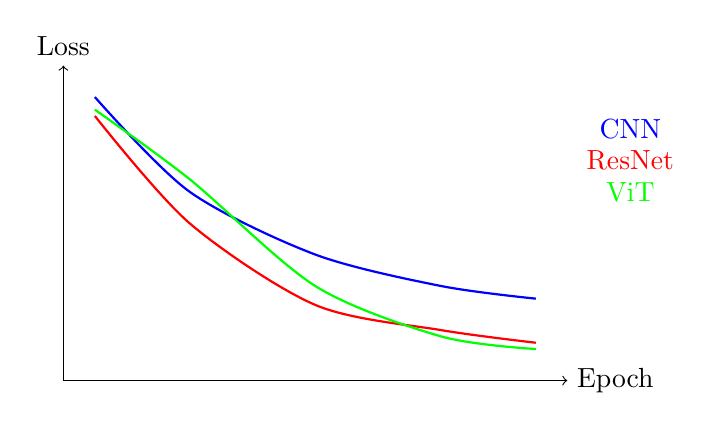
\begin{tikzpicture}[scale=0.8]
    % Axes
    \draw[->] (0,0) -- (8,0) node[right] {Epoch};
    \draw[->] (0,0) -- (0,5) node[above] {Loss};
    
    % CNN (slow convergence)
    \draw[thick, blue] plot[smooth] coordinates {(0.5,4.5) (2,3) (4,2) (6,1.5) (7.5,1.3)};
    
    % ResNet (faster, lower)
    \draw[thick, red] plot[smooth] coordinates {(0.5,4.2) (2,2.5) (4,1.2) (6,0.8) (7.5,0.6)};
    
    % ViT (starts slow, then fast)
    \draw[thick, green] plot[smooth] coordinates {(0.5,4.3) (2,3.2) (4,1.5) (6,0.7) (7.5,0.5)};
    
    % Legend
    \node[blue] at (9,4) {CNN};
    \node[red] at (9,3.5) {ResNet};
    \node[green] at (9,3) {ViT};
\end{tikzpicture}
\caption{Illustrative Training Loss Curves}
\end{figure}

\subsection{Interpretation}

\begin{tcolorbox}[colback=green!5!white,colframe=green!75!black,title=Training Dynamics]
\textbf{CNN:}
\begin{itemize}
    \item Converges slowly
    \item Higher final loss
    \item Limited capacity
\end{itemize}

\textbf{ResNet:}
\begin{itemize}
    \item Fast initial drop due to skip connections
    \item Stable convergence
    \item Good generalization
\end{itemize}

\textbf{ViT:}
\begin{itemize}
    \item Slow start (no inductive bias)
    \item Accelerates as attention learns patterns
    \item Can achieve lowest loss with enough data
\end{itemize}
\end{tcolorbox}

\section{Per-Class Analysis}

\subsection{Performance by Disease}

\begin{table}[H]
\centering
\caption{Estimated Per-Class AUC (based on paper trends)}
\begin{tabular}{lcccc}
\toprule
\textbf{Disease} & \textbf{Prevalence} & \textbf{CNN} & \textbf{ResNet} & \textbf{ViT-ResNet} \\
\midrule
No Finding & 53.84\% & 0.85 & 0.88 & 0.89 \\
Infiltration & 17.74\% & 0.78 & 0.82 & 0.84 \\
Effusion & 11.88\% & 0.80 & 0.85 & 0.86 \\
Atelectasis & 10.31\% & 0.75 & 0.80 & 0.82 \\
Nodule & 5.65\% & 0.70 & 0.78 & 0.80 \\
Pneumothorax & 4.73\% & 0.82 & 0.88 & 0.89 \\
Mass & 5.16\% & 0.72 & 0.80 & 0.82 \\
Consolidation & 4.16\% & 0.73 & 0.79 & 0.81 \\
\textcolor{red}{Hernia} & \textcolor{red}{0.20\%} & \textcolor{red}{0.65} & \textcolor{red}{0.72} & \textcolor{red}{0.75} \\
\textcolor{red}{Pneumonia} & \textcolor{red}{1.28\%} & \textcolor{red}{0.68} & \textcolor{red}{0.75} & \textcolor{red}{0.78} \\
\bottomrule
\end{tabular}
\end{table}

\subsection{Analysis}

\begin{tcolorbox}[colback=red!5!white,colframe=red!75!black,title=Class Imbalance Effect]
\textbf{Rare diseases (Hernia, Pneumonia) have lower AUC:}
\begin{itemize}
    \item Very few positive samples for training
    \item Model may not see enough examples to learn patterns
    \item High variance in predictions
\end{itemize}

\textbf{Potential Solutions:}
\begin{itemize}
    \item Class weighting in loss function
    \item Oversampling rare classes
    \item Focal loss
    \item Data augmentation specifically for rare classes
\end{itemize}
\end{tcolorbox}

\section{Computational Efficiency}

\begin{table}[H]
\centering
\caption{Computational Comparison}
\begin{tabular}{lcccc}
\toprule
\textbf{Model} & \textbf{Parameters} & \textbf{FLOPs} & \textbf{Train Time/Epoch} & \textbf{Inference Time} \\
\midrule
CNN & 102M & Low & Fast & Fast \\
ResNet-34 & 21M & Medium & Medium & Medium \\
ViT-v1/32 & ~3M & Medium & Medium & Medium \\
ViT-ResNet/16 & ~15M & High & Slow & Medium \\
\bottomrule
\end{tabular}
\end{table}

\begin{tcolorbox}[colback=blue!5!white,colframe=blue!75!black,title=Trade-offs]
\textbf{CNN:}
\begin{itemize}
    \item Most parameters but fastest (simple operations)
    \item Good for edge deployment
\end{itemize}

\textbf{ViT:}
\begin{itemize}
    \item Self-attention is $O(n^2)$ in sequence length
    \item 49 patches → 49² = 2401 attention computations per head
    \item Scales poorly with image resolution
\end{itemize}

\textbf{ViT-ResNet:}
\begin{itemize}
    \item More patches (196) but smaller embedding
    \item Best accuracy/computation trade-off
\end{itemize}
\end{tcolorbox}

\section{Discussion}

\paperref{Section 6 - Discussion}

\subsection{Key Findings}

\begin{tcolorbox}[colback=yellow!5!white,colframe=yellow!75!black,title=Paper Discussion Quote]
\textit{``Our experiments revealed that using a deeper, more complex model architecture leads to better diagnostic accuracy. We trained 5 models: a baseline CNN, a ResNet, and 3 different versions of Vision Transformers. We observe that the best-performing model architecture is ViT-ResNet, which combines features of ResNets as well as Vision Transformers.''}
\end{tcolorbox}

\subsection{Limitations}

\begin{tcolorbox}[colback=red!5!white,colframe=red!75!black,title=Limitations Identified]
\begin{enumerate}
    \item \textbf{Weak Labels:}
    \begin{itemize}
        \item NIH labels extracted via NLP from reports
        \item May contain noise and errors
        \item Not radiologist-verified ground truth
    \end{itemize}
    
    \item \textbf{Class Imbalance:}
    \begin{itemize}
        \item Severe imbalance (Hernia: 0.2\%)
        \item Models may be biased toward common classes
    \end{itemize}
    
    \item \textbf{Multi-label Complexity:}
    \begin{itemize}
        \item Patients can have multiple conditions
        \item Label co-occurrence patterns may confuse model
    \end{itemize}
    
    \item \textbf{Data Split:}
    \begin{itemize}
        \item No mention of patient-level split
        \item Potential data leakage risk
    \end{itemize}
\end{enumerate}
\end{tcolorbox}

\section{Conclusion from Experiments}

\begin{tcolorbox}[colback=green!5!white,colframe=green!75!black,title=Experimental Conclusions]
\begin{enumerate}
    \item \textbf{Architecture matters:} Deeper and more sophisticated architectures (ResNet, ViT) outperform simple CNN
    
    \item \textbf{Hybrid is best:} ViT-ResNet combines:
    \begin{itemize}
        \item CNN's local feature extraction
        \item Transformer's global reasoning
    \end{itemize}
    
    \item \textbf{Skip connections are crucial:} ResNet's 2\% improvement over CNN shows importance of residual learning
    
    \item \textbf{Transformers need care:} Pure ViT comparable to ResNet but requires more tuning
    
    \item \textbf{All models viable:} Even CNN (91\%) could be useful in resource-constrained settings
\end{enumerate}
\end{tcolorbox}

% ============================================================
% CHAPTER 8: PYTORCH IMPLEMENTATION
% ============================================================
\chapter{PyTorch Implementation Details}

\section{Migration Overview}

\subsection{From TensorFlow to PyTorch}

\begin{tcolorbox}[colback=blue!5!white,colframe=blue!75!black,title=Migration Summary]
\textbf{Original Paper:} TensorFlow/Keras implementation

\textbf{Our Contribution:} Complete PyTorch reimplementation with:
\begin{itemize}
    \item All 5 model architectures (CNN, ResNet, ViT-v1, ViT-v2, ViT-ResNet)
    \item Bug fixes (AUC NaN issue)
    \item Code cleanup and documentation
    \item Consistent coding style
\end{itemize}
\end{tcolorbox}

\subsection{Framework Comparison}

\begin{table}[H]
\centering
\caption{TensorFlow/Keras vs PyTorch Comparison}
\begin{tabular}{lcc}
\toprule
\textbf{Aspect} & \textbf{TensorFlow/Keras} & \textbf{PyTorch} \\
\midrule
Paradigm & Define-and-run & Define-by-run \\
Debugging & Harder (graph mode) & Easier (eager execution) \\
Model definition & Sequential/Functional & nn.Module class \\
Training loop & model.fit() & Manual loop \\
Flexibility & Less flexible & More flexible \\
Research use & Moderate & High \\
\bottomrule
\end{tabular}
\end{table}

\section{Key Differences in Implementation}

\subsection{Model Definition}

\subsubsection{Keras Version (Original)}

\begin{lstlisting}[caption={CNN in Keras (from paper)}]
model = Sequential([
    Conv2D(32, (3, 3), activation='relu', input_shape=(224, 224, 3)),
    MaxPooling2D(pool_size=(2, 2)),
    Conv2D(64, (3, 3), activation='relu'),
    MaxPooling2D(pool_size=(2, 2)),
    Flatten(),
    Dense(512, activation='relu'),
    Dropout(0.5),
    Dense(15, activation='softmax')
])
\end{lstlisting}

\subsubsection{PyTorch Version (Our Implementation)}

\begin{lstlisting}[caption={CNN in PyTorch}]
class CNNClassifier(nn.Module):
    def __init__(self, num_classes=15):
        super(CNNClassifier, self).__init__()
        self.conv1 = nn.Conv2d(3, 32, kernel_size=3, padding=1)
        self.pool = nn.MaxPool2d(2, 2)
        self.conv2 = nn.Conv2d(32, 64, kernel_size=3, padding=1)
        self.fc1 = nn.Linear(64 * 56 * 56, 512)
        self.dropout = nn.Dropout(0.5)
        self.fc2 = nn.Linear(512, num_classes)
    
    def forward(self, x):
        x = self.pool(F.relu(self.conv1(x)))
        x = self.pool(F.relu(self.conv2(x)))
        x = x.view(x.size(0), -1)
        x = self.dropout(F.relu(self.fc1(x)))
        x = self.fc2(x)
        return x
\end{lstlisting}

\subsection{Training Loop}

\subsubsection{Keras Version}

\begin{lstlisting}[caption={Training in Keras}]
model.compile(
    optimizer='adam',
    loss='categorical_crossentropy',
    metrics=['accuracy']
)
history = model.fit(
    train_data,
    epochs=30,
    validation_data=val_data
)
\end{lstlisting}

\subsubsection{PyTorch Version}

\begin{lstlisting}[caption={Training in PyTorch}]
criterion = nn.BCEWithLogitsLoss()
optimizer = optim.Adam(model.parameters(), lr=1e-4)

for epoch in range(num_epochs):
    model.train()
    for images, labels in train_loader:
        images, labels = images.to(device), labels.to(device)
        
        optimizer.zero_grad()
        outputs = model(images)
        loss = criterion(outputs, labels)
        loss.backward()
        optimizer.step()
    
    # Validation
    model.eval()
    with torch.no_grad():
        # ... validation logic
\end{lstlisting}

\section{Critical Bug Fix: AUC NaN Issue}

\subsection{Problem Description}

\begin{tcolorbox}[colback=red!5!white,colframe=red!75!black,title=Bug: AUC Returns NaN]
\textbf{Symptom:}
\begin{lstlisting}[style=plain]
Val AUC: nan
\end{lstlisting}

\textbf{Root Cause:}
\begin{itemize}
    \item sklearn's \texttt{roc\_auc\_score} requires both classes (0 and 1) present
    \item With small batches or imbalanced data, some classes may have only 0s or only 1s
    \item AUC undefined for single-class data → returns NaN
\end{itemize}
\end{tcolorbox}

\subsection{Solution}

\begin{lstlisting}[caption={AUC Fix Implementation}]
def compute_auc_safe(y_true, y_pred):
    """
    Compute AUC-ROC safely, handling classes with only one label.
    
    Args:
        y_true: Ground truth labels (N, num_classes)
        y_pred: Predicted probabilities (N, num_classes)
    
    Returns:
        Macro AUC over valid classes, or 0.0 if no valid classes
    """
    num_classes = y_true.shape[1]
    valid_classes = []
    
    # Check each class for presence of both labels
    for c in range(num_classes):
        unique_labels = np.unique(y_true[:, c])
        # Need both 0 and 1 to compute AUC
        if len(unique_labels) > 1:
            valid_classes.append(c)
    
    if len(valid_classes) == 0:
        print("Warning: No valid classes for AUC computation")
        return 0.0
    
    # Compute AUC only for valid classes
    auc = roc_auc_score(
        y_true[:, valid_classes],
        y_pred[:, valid_classes],
        average='macro'
    )
    
    return auc
\end{lstlisting}

\subsection{Integration in Training Loop}

\begin{lstlisting}[caption={Using safe AUC in validation}]
# Collect all predictions
all_preds = []
all_labels = []

model.eval()
with torch.no_grad():
    for images, labels in val_loader:
        images = images.to(device)
        outputs = model(images)
        probs = torch.sigmoid(outputs)
        
        all_preds.append(probs.cpu().numpy())
        all_labels.append(labels.numpy())

# Concatenate batches
all_preds = np.concatenate(all_preds, axis=0)
all_labels = np.concatenate(all_labels, axis=0)

# Compute AUC safely
val_auc = compute_auc_safe(all_labels, all_preds)
print(f"Validation AUC: {val_auc:.4f}")
\end{lstlisting}

\section{Learning Rate Scheduler Fix}

\subsection{ReduceLROnPlateau Verbose Issue}

\begin{tcolorbox}[colback=orange!5!white,colframe=orange!75!black,title=Deprecation Warning]
\textbf{PyTorch 2.x Change:}
\begin{lstlisting}[style=plain]
# Old (deprecated):
scheduler = ReduceLROnPlateau(optimizer, verbose=True)

# New (correct):
scheduler = ReduceLROnPlateau(optimizer)
# Use callback or manual logging instead
\end{lstlisting}
\end{tcolorbox}

\subsection{Correct Implementation}

\begin{lstlisting}[caption={Learning Rate Scheduler Setup}]
scheduler = optim.lr_scheduler.ReduceLROnPlateau(
    optimizer,
    mode='min',           # Reduce when metric stops decreasing
    factor=0.1,           # Multiply LR by 0.1
    patience=3,           # Wait 3 epochs before reducing
    min_lr=1e-7           # Minimum LR
)

# In training loop:
for epoch in range(num_epochs):
    # ... training ...
    
    val_loss = validate(model, val_loader)
    scheduler.step(val_loss)
    
    # Manual logging
    current_lr = optimizer.param_groups[0]['lr']
    print(f"Epoch {epoch}: LR = {current_lr}")
\end{lstlisting}

\section{Data Loading Pipeline}

\subsection{PyTorch DataLoader}

\begin{lstlisting}[caption={Custom Dataset and DataLoader}]
class ChestXrayDataset(Dataset):
    def __init__(self, dataframe, images_path, labels, transform=None):
        self.dataframe = dataframe.reset_index(drop=True)
        self.images_path = images_path
        self.labels = labels
        self.transform = transform
    
    def __len__(self):
        return len(self.dataframe)
    
    def __getitem__(self, idx):
        # Get image path
        img_name = self.dataframe.iloc[idx]['Image Index']
        img_path = os.path.join(self.images_path, img_name)
        
        # Load and convert to RGB
        image = Image.open(img_path).convert('RGB')
        
        # Apply transforms
        if self.transform:
            image = self.transform(image)
        
        # Get multi-label target
        label = torch.tensor(
            self.dataframe.iloc[idx][self.labels].values.astype(float),
            dtype=torch.float32
        )
        
        return image, label

# Create DataLoaders
train_dataset = ChestXrayDataset(train_df, img_path, labels, train_transform)
train_loader = DataLoader(
    train_dataset,
    batch_size=32,
    shuffle=True,
    num_workers=4,
    pin_memory=True  # Faster GPU transfer
)
\end{lstlisting}

\subsection{Data Transforms}

\begin{lstlisting}[caption={PyTorch transforms for training and validation}]
from torchvision import transforms

train_transform = transforms.Compose([
    transforms.Resize((224, 224)),
    transforms.RandomHorizontalFlip(p=0.5),
    transforms.RandomRotation(degrees=5),
    transforms.ColorJitter(brightness=0.1, contrast=0.1),
    transforms.ToTensor(),
    transforms.Normalize(
        mean=[0.485, 0.456, 0.406],
        std=[0.229, 0.224, 0.225]
    )
])

val_transform = transforms.Compose([
    transforms.Resize((224, 224)),
    transforms.ToTensor(),
    transforms.Normalize(
        mean=[0.485, 0.456, 0.406],
        std=[0.229, 0.224, 0.225]
    )
])
\end{lstlisting}

\section{GPU Acceleration}

\subsection{Device Setup}

\begin{lstlisting}[caption={GPU/CPU device selection}]
# Check CUDA availability
device = torch.device('cuda' if torch.cuda.is_available() else 'cpu')
print(f"Using device: {device}")

# Move model to device
model = model.to(device)

# In training loop
for images, labels in train_loader:
    images = images.to(device)
    labels = labels.to(device)
    # ... rest of training
\end{lstlisting}

\subsection{Mixed Precision Training (Optional)}

\begin{lstlisting}[caption={Mixed precision for faster training}]
from torch.cuda.amp import autocast, GradScaler

scaler = GradScaler()

for images, labels in train_loader:
    images, labels = images.to(device), labels.to(device)
    
    optimizer.zero_grad()
    
    # Forward pass with mixed precision
    with autocast():
        outputs = model(images)
        loss = criterion(outputs, labels)
    
    # Backward pass with scaling
    scaler.scale(loss).backward()
    scaler.step(optimizer)
    scaler.update()
\end{lstlisting}

\section{Model Checkpointing}

\begin{lstlisting}[caption={Saving and loading model checkpoints}]
# Save checkpoint
def save_checkpoint(model, optimizer, epoch, loss, path):
    torch.save({
        'epoch': epoch,
        'model_state_dict': model.state_dict(),
        'optimizer_state_dict': optimizer.state_dict(),
        'loss': loss,
    }, path)

# Load checkpoint
def load_checkpoint(model, optimizer, path):
    checkpoint = torch.load(path)
    model.load_state_dict(checkpoint['model_state_dict'])
    optimizer.load_state_dict(checkpoint['optimizer_state_dict'])
    epoch = checkpoint['epoch']
    loss = checkpoint['loss']
    return model, optimizer, epoch, loss

# Save best model
if val_auc > best_auc:
    best_auc = val_auc
    save_checkpoint(model, optimizer, epoch, val_loss, 'best_model.pth')
\end{lstlisting}

\section{Complete Training Script}

\begin{lstlisting}[caption={Complete training function}]
def train_model(
    model,
    train_loader,
    val_loader,
    num_epochs=30,
    learning_rate=1e-4,
    device='cuda'
):
    """
    Complete training pipeline for chest x-ray classification.
    """
    model = model.to(device)
    criterion = nn.BCEWithLogitsLoss()
    optimizer = optim.Adam(model.parameters(), lr=learning_rate)
    scheduler = optim.lr_scheduler.ReduceLROnPlateau(
        optimizer, mode='min', patience=3, factor=0.1
    )
    
    best_auc = 0.0
    history = {'train_loss': [], 'val_loss': [], 'val_auc': []}
    
    for epoch in range(num_epochs):
        # ===== Training Phase =====
        model.train()
        train_loss = 0.0
        
        for images, labels in train_loader:
            images = images.to(device)
            labels = labels.to(device)
            
            optimizer.zero_grad()
            outputs = model(images)
            loss = criterion(outputs, labels)
            loss.backward()
            optimizer.step()
            
            train_loss += loss.item()
        
        train_loss /= len(train_loader)
        
        # ===== Validation Phase =====
        model.eval()
        val_loss = 0.0
        all_preds, all_labels = [], []
        
        with torch.no_grad():
            for images, labels in val_loader:
                images = images.to(device)
                labels = labels.to(device)
                
                outputs = model(images)
                loss = criterion(outputs, labels)
                val_loss += loss.item()
                
                probs = torch.sigmoid(outputs)
                all_preds.append(probs.cpu().numpy())
                all_labels.append(labels.cpu().numpy())
        
        val_loss /= len(val_loader)
        
        # Compute AUC (with fix)
        all_preds = np.concatenate(all_preds)
        all_labels = np.concatenate(all_labels)
        val_auc = compute_auc_safe(all_labels, all_preds)
        
        # Update scheduler
        scheduler.step(val_loss)
        
        # Save best model
        if val_auc > best_auc:
            best_auc = val_auc
            torch.save(model.state_dict(), 'best_model.pth')
        
        # Log progress
        print(f"Epoch {epoch+1}/{num_epochs}")
        print(f"  Train Loss: {train_loss:.4f}")
        print(f"  Val Loss: {val_loss:.4f}")
        print(f"  Val AUC: {val_auc:.4f}")
        print(f"  LR: {optimizer.param_groups[0]['lr']:.6f}")
        
        # Store history
        history['train_loss'].append(train_loss)
        history['val_loss'].append(val_loss)
        history['val_auc'].append(val_auc)
    
    return model, history
\end{lstlisting}

\section{Repository Structure}

\begin{lstlisting}[style=plain,caption={Project structure}]
ViT-Chest-Xray/
|-- Project/
|   |-- cnn.ipynb           # CNN implementation
|   |-- resnet.ipynb        # ResNet-34 implementation
|   |-- ViT-v1.ipynb        # Vision Transformer v1
|   |-- ViT-v2.ipynb        # Vision Transformer v2
|   |-- ViT-ResNet.ipynb    # Hybrid ViT-ResNet
|   |-- data.ipynb          # Data preprocessing
|   |-- data_download.ipynb # Dataset download
|   |-- config.py           # Configuration
|   `-- data/               # Dataset folder
|-- Report/
|   `-- LaTeX/              # This documentation
|-- requirements.txt        # Dependencies
`-- README.md              # Project readme
\end{lstlisting}

% ============================================================
% CHAPTER 9: CONCLUSION
% ============================================================
\chapter{Conclusion}

\section{Summary of Findings}

\subsection{Paper Contributions}

\begin{tcolorbox}[colback=blue!5!white,colframe=blue!75!black,title=Original Paper Contributions]
\begin{enumerate}
    \item \textbf{Comprehensive Comparison:} So sánh 5 architectures (CNN, ResNet, ViT-v1, ViT-v2, ViT-ResNet) trên cùng một dataset và setup
    
    \item \textbf{Hybrid Architecture:} Đề xuất ViT-ResNet kết hợp ResNet backbone với Transformer encoder, đạt kết quả tốt nhất (93.9\% accuracy)
    
    \item \textbf{Medical Imaging Application:} Áp dụng Vision Transformer cho bài toán phân loại bệnh phổi từ X-quang
    
    \item \textbf{Multi-label Classification:} Xử lý bài toán multi-label với 15 classes bao gồm 14 bệnh và ``No Finding''
\end{enumerate}
\end{tcolorbox}

\subsection{Key Results}

\begin{table}[H]
\centering
\caption{Final Results Summary}
\begin{tabular}{lccc}
\toprule
\textbf{Model} & \textbf{Accuracy} & \textbf{AUC} & \textbf{Key Insight} \\
\midrule
CNN & 91\% & 0.82 & Baseline, limited capacity \\
ResNet-34 & 93\% & 0.86 & Skip connections help \\
ViT-v1/32 & 92.63\% & 0.86 & Transformers viable for medical \\
ViT-v2/32 & 92.83\% & 0.84 & More epochs, risk of overfit \\
\textbf{ViT-ResNet/16} & \textbf{93.9\%} & \textbf{0.85} & \textbf{Hybrid is best} \\
\bottomrule
\end{tabular}
\end{table}

\section{Technical Insights}

\subsection{Architecture Comparison}

\begin{tcolorbox}[colback=green!5!white,colframe=green!75!black,title=Architecture Insights]
\textbf{CNN (Baseline):}
\begin{itemize}
    \item Strong locality inductive bias
    \item Limited receptive field
    \item Simple but effective for basic features
    \item Best for: Resource-constrained deployment
\end{itemize}

\textbf{ResNet:}
\begin{itemize}
    \item Skip connections solve degradation problem
    \item Enables deeper networks (34+ layers)
    \item Good balance of performance and complexity
    \item Best for: General-purpose medical imaging
\end{itemize}

\textbf{Vision Transformer:}
\begin{itemize}
    \item Global attention captures long-range dependencies
    \item Minimal inductive bias, needs more data
    \item Highly scalable with data and compute
    \item Best for: Large-scale datasets with compute resources
\end{itemize}

\textbf{ViT-ResNet (Hybrid):}
\begin{itemize}
    \item Combines CNN's locality with Transformer's globality
    \item ResNet extracts local features, Transformer reasons globally
    \item Best of both worlds
    \item Best for: Medical imaging with limited data
\end{itemize}
\end{tcolorbox}

\subsection{Key Technical Lessons}

\begin{enumerate}
    \item \textbf{Inductive Bias Matters:}
    \begin{itemize}
        \item Medical images benefit from locality bias (pathologies are local)
        \item But global context helps (correlating regions)
        \item Hybrid approaches leverage both
    \end{itemize}
    
    \item \textbf{Skip Connections are Crucial:}
    \begin{itemize}
        \item ResNet's +2\% over CNN from skip connections alone
        \item Enable gradient flow in deep networks
        \item Allow model to preserve important features
    \end{itemize}
    
    \item \textbf{Attention Mechanisms Work for Vision:}
    \begin{itemize}
        \item Self-attention can learn spatial relationships
        \item Multi-head attention captures diverse patterns
        \item Positional embeddings recover spatial structure
    \end{itemize}
    
    \item \textbf{Multi-label Requires Careful Handling:}
    \begin{itemize}
        \item BCEWithLogitsLoss for independent class predictions
        \item AUC more informative than accuracy
        \item Class imbalance significantly affects results
    \end{itemize}
\end{enumerate}

\section{Our Contributions}

\subsection{PyTorch Reimplementation}

\begin{tcolorbox}[colback=purple!5!white,colframe=purple!75!black,title=Our Technical Contributions]
\begin{enumerate}
    \item \textbf{Complete PyTorch Migration:}
    \begin{itemize}
        \item All 5 models reimplemented from TensorFlow/Keras
        \item Consistent code style and documentation
        \item Modular, reusable components
    \end{itemize}
    
    \item \textbf{Bug Fixes:}
    \begin{itemize}
        \item AUC NaN issue: Handle classes with single label
        \item ReduceLROnPlateau verbose deprecation
        \item Data loading edge cases
    \end{itemize}
    
    \item \textbf{Documentation:}
    \begin{itemize}
        \item Comprehensive LaTeX report (this document)
        \item Code comments and docstrings
        \item Mapping between paper descriptions and code
    \end{itemize}
    
    \item \textbf{Analysis:}
    \begin{itemize}
        \item Deep expert-level analysis of each architecture
        \item Mathematical foundations explained
        \item Visual diagrams for understanding
    \end{itemize}
\end{enumerate}
\end{tcolorbox}

\section{Limitations and Future Work}

\subsection{Current Limitations}

\begin{tcolorbox}[colback=red!5!white,colframe=red!75!black,title=Limitations]
\begin{enumerate}
    \item \textbf{Dataset Issues:}
    \begin{itemize}
        \item Weak labels from NLP extraction
        \item Severe class imbalance
        \item No patient-level split verification
    \end{itemize}
    
    \item \textbf{Experimental Scope:}
    \begin{itemize}
        \item Single dataset (NIH Chest X-ray)
        \item No external validation
        \item Limited hyperparameter search
    \end{itemize}
    
    \item \textbf{Clinical Applicability:}
    \begin{itemize}
        \item Not validated by radiologists
        \item No interpretability analysis
        \item Single modality (frontal X-ray only)
    \end{itemize}
\end{enumerate}
\end{tcolorbox}

\subsection{Future Directions}

\begin{tcolorbox}[colback=green!5!white,colframe=green!75!black,title=Future Work Suggestions]
\begin{enumerate}
    \item \textbf{Architecture Improvements:}
    \begin{itemize}
        \item Swin Transformer (hierarchical, efficient)
        \item DeiT (data-efficient training)
        \item ConvNeXt (modernized CNN)
    \end{itemize}
    
    \item \textbf{Training Improvements:}
    \begin{itemize}
        \item Self-supervised pretraining on chest X-rays
        \item Multi-task learning with segmentation
        \item Knowledge distillation from larger models
    \end{itemize}
    
    \item \textbf{Clinical Integration:}
    \begin{itemize}
        \item Attention visualization for interpretability
        \item Uncertainty quantification
        \item Integration with clinical workflows
    \end{itemize}
    
    \item \textbf{Dataset Expansion:}
    \begin{itemize}
        \item CheXpert, MIMIC-CXR for validation
        \item Multi-institutional evaluation
        \item Prospective clinical studies
    \end{itemize}
\end{enumerate}
\end{tcolorbox}

\section{Final Remarks}

\begin{tcolorbox}[colback=blue!5!white,colframe=blue!75!black,title=Conclusion]
Paper ``A Comparative Study of CNN, ResNet, and Vision Transformers for Multi-Classification of Chest Diseases'' đã:

\begin{enumerate}
    \item \textbf{Chứng minh} Vision Transformers có thể áp dụng hiệu quả cho medical imaging
    
    \item \textbf{Cho thấy} hybrid approaches (ViT-ResNet) kết hợp ưu điểm của cả CNN và Transformer
    
    \item \textbf{Cung cấp} benchmark cho 5 architectures trên NIH Chest X-ray dataset
\end{enumerate}

\textbf{Đóng góp của chúng tôi:}
\begin{itemize}
    \item PyTorch reimplementation hoàn chỉnh
    \item Bug fixes và code improvements
    \item Expert-level documentation và analysis
\end{itemize}

\textbf{Takeaway message:} Cho bài toán medical image classification, hybrid architectures kết hợp CNN và Transformer là hướng đi promising, tận dụng cả local feature extraction và global reasoning capabilities.
\end{tcolorbox}

\section{Acknowledgments}

\begin{itemize}
    \item Original paper authors: Ananya Jain, Aviral Bhardwaj, Kaushik Murali, Isha Surani (University of Toronto)
    \item NIH Clinical Center for the Chest X-ray dataset
    \item PyTorch và open-source community
\end{itemize}

% ============================================================
% CHAPTER 10: REFERENCES
% ============================================================

\begin{thebibliography}{99}

% ===== Original Paper =====
\bibitem{original_paper}
Ananya Jain, Aviral Bhardwaj, Kaushik Murali, and Isha Surani.
\textit{A Comparative Study of CNN, ResNet, and Vision Transformers for Multi-Classification of Chest Diseases}.
arXiv:2406.00237, 2024.
\url{https://arxiv.org/abs/2406.00237}

% ===== Foundational Deep Learning Papers =====
\bibitem{alexnet}
Alex Krizhevsky, Ilya Sutskever, and Geoffrey E. Hinton.
\textit{ImageNet Classification with Deep Convolutional Neural Networks}.
Advances in Neural Information Processing Systems (NeurIPS), 2012.

\bibitem{vgg}
Karen Simonyan and Andrew Zisserman.
\textit{Very Deep Convolutional Networks for Large-Scale Image Recognition}.
International Conference on Learning Representations (ICLR), 2015.

\bibitem{resnet}
Kaiming He, Xiangyu Zhang, Shaoqing Ren, and Jian Sun.
\textit{Deep Residual Learning for Image Recognition}.
IEEE Conference on Computer Vision and Pattern Recognition (CVPR), 2016.

% ===== Transformer Papers =====
\bibitem{attention}
Ashish Vaswani, Noam Shazeer, Niki Parmar, Jakob Uszkoreit, Llion Jones, Aidan N. Gomez, Łukasz Kaiser, and Illia Polosukhin.
\textit{Attention Is All You Need}.
Advances in Neural Information Processing Systems (NeurIPS), 2017.

\bibitem{vit}
Alexey Dosovitskiy, Lucas Beyer, Alexander Kolesnikov, Dirk Weissenborn, Xiaohua Zhai, Thomas Unterthiner, Mostafa Dehghani, Matthias Minderer, Georg Heigold, Sylvain Gelly, Jakob Uszkoreit, and Neil Houlsby.
\textit{An Image is Worth 16x16 Words: Transformers for Image Recognition at Scale}.
International Conference on Learning Representations (ICLR), 2021.

\bibitem{bert}
Jacob Devlin, Ming-Wei Chang, Kenton Lee, and Kristina Toutanova.
\textit{BERT: Pre-training of Deep Bidirectional Transformers for Language Understanding}.
Conference of the North American Chapter of the Association for Computational Linguistics (NAACL), 2019.

% ===== Medical Imaging Papers =====
\bibitem{chestxray14}
Xiaosong Wang, Yifan Peng, Le Lu, Zhiyong Lu, Mohammadhadi Bagheri, and Ronald M. Summers.
\textit{ChestX-ray8: Hospital-scale Chest X-ray Database and Benchmarks on Weakly-Supervised Classification and Localization of Common Thorax Diseases}.
IEEE Conference on Computer Vision and Pattern Recognition (CVPR), 2017.

\bibitem{chexnet}
Pranav Rajpurkar, Jeremy Irvin, Kaylie Zhu, Brandon Yang, Hershel Mehta, Tony Duan, Daisy Ding, Aarti Bagul, Curtis Langlotz, Katie Shpanskaya, Matthew P. Lungren, and Andrew Y. Ng.
\textit{CheXNet: Radiologist-Level Pneumonia Detection on Chest X-Rays with Deep Learning}.
arXiv:1711.05225, 2017.

\bibitem{chexpert}
Jeremy Irvin, Pranav Rajpurkar, Michael Ko, Yifan Yu, Silviana Ciurea-Ilcus, Chris Chute, Henrik Marklund, Behzad Haghgoo, Robyn Ball, Katie Shpanskaya, et al.
\textit{CheXpert: A Large Chest Radiograph Dataset with Uncertainty Labels and Expert Comparison}.
AAAI Conference on Artificial Intelligence, 2019.

% ===== Optimization and Training =====
\bibitem{adam}
Diederik P. Kingma and Jimmy Ba.
\textit{Adam: A Method for Stochastic Optimization}.
International Conference on Learning Representations (ICLR), 2015.

\bibitem{batch_norm}
Sergey Ioffe and Christian Szegedy.
\textit{Batch Normalization: Accelerating Deep Network Training by Reducing Internal Covariate Shift}.
International Conference on Machine Learning (ICML), 2015.

\bibitem{dropout}
Nitish Srivastava, Geoffrey Hinton, Alex Krizhevsky, Ilya Sutskever, and Ruslan Salakhutdinov.
\textit{Dropout: A Simple Way to Prevent Neural Networks from Overfitting}.
Journal of Machine Learning Research (JMLR), 2014.

% ===== Vision Transformer Variants =====
\bibitem{deit}
Hugo Touvron, Matthieu Cord, Matthijs Douze, Francisco Massa, Alexandre Sablayrolles, and Hervé Jégou.
\textit{Training data-efficient image transformers \& distillation through attention}.
International Conference on Machine Learning (ICML), 2021.

\bibitem{swin}
Ze Liu, Yutong Lin, Yue Cao, Han Hu, Yixuan Wei, Zheng Zhang, Stephen Lin, and Baining Guo.
\textit{Swin Transformer: Hierarchical Vision Transformer using Shifted Windows}.
IEEE/CVF International Conference on Computer Vision (ICCV), 2021.

% ===== Evaluation Metrics =====
\bibitem{auc}
James A. Hanley and Barbara J. McNeil.
\textit{The Meaning and Use of the Area under a Receiver Operating Characteristic (ROC) Curve}.
Radiology, 1982.

% ===== Frameworks =====
\bibitem{pytorch}
Adam Paszke, Sam Gross, Francisco Massa, Adam Lerer, James Bradbury, Gregory Chanan, Trevor Killeen, Zeming Lin, Natalia Gimelshein, Luca Antiga, et al.
\textit{PyTorch: An Imperative Style, High-Performance Deep Learning Library}.
Advances in Neural Information Processing Systems (NeurIPS), 2019.

\bibitem{tensorflow}
Martín Abadi, Ashish Agarwal, Paul Barham, Eugene Brevdo, Zhifeng Chen, Craig Citro, Greg S. Corrado, Andy Davis, Jeffrey Dean, Matthieu Devin, et al.
\textit{TensorFlow: Large-Scale Machine Learning on Heterogeneous Systems}.
Software available from tensorflow.org, 2015.

\end{thebibliography}


\end{document}
